\section{Model Comparison}\label{sec:comparisons}

We now apply the observational constraints from Section~\ref{sec:observations} to the models described in Section~\ref{sec:models}.  We have shown visually how models pass or fail in Figures~\ref{fig:passfail_sz}, \ref{fig:passfail_va}, and \ref{fig:passfail_sed}.  For each of these figures, the left panel is from the best-bet region (see Section~\ref{sec:discussions}) that passes all but the variability constraints, and the right panel is one of the failed models.

\subsection{Fiducial Models}\label{subsec:thermal}

We start with the fiducial models.  Recall that these have aligned (prograde or retrograde) accretion flows, thermal eDFs, and electron temperature assigned according to the $\Rh$ model, as in \citetalias{M87PaperV}.  This selection includes the \kharma, \bhac, and \hamr model sets listed near the top of Table~\ref{tab:radiativemodels}.  

A full set of pass/fail plots, showing how the three, redundant fiducial models fare, is provided in Appendix \ref{app:tables}. Table ~\ref{tab:passfraction_thermal} summarizes the fraction of fiducial \kharma, \bhac, and \hamr models that pass each constraint. 

\begin{table*}
\caption{Summary of constraints and passing fractions for \kharma, \bhac, and \hamr thermal models}
\centering
\begin{tabular}{l|l|ccc}
\hline
Constraint & Description & \kharma	&	\bhac	&	\hamr \\
\hline
230\,GHz size	        &	&	0.98	&	0.98   &	1.0		\\
lc varability	        &	&	0.20	&	0.27   &	0.07	\\
4G$\lambda$ variability	&	&	0.60	&	0.72   &	0.39	\\
Null location	        &	&	0.84	&	0.83   &	0.80	\\
M-ring diameter	        &	&	0.67	&	0.65   &	0.61	\\
M-ring width	        &	&	0.35	&	0.21   &	0.32	\\
M-ring asym.	        &	&	0.94	&	0.95   &	0.99	\\
86\GHz size	            &	&	0.62	&	0.59   &	0.46	\\
86\GHz flux	            &	&	0.75	&	0.68   &	0.62	\\
2.2\um flux             &	&	0.59	&	0.55   &	0.80	\\
X-ray flux		        &	&	0.46	&	0.70   &	0.35	\\
\hline
\end{tabular}
\label{tab:passfraction_thermal}
\end{table*} 

\subsubsection{EHT Constraints}

How do the models fare when compared to the EHT data alone, using the size, null location, and \mring fitting constraints?  The size constraint is simple but uninformative: only a few face-on, $\Rh = 1$ models fail the test.  The null location test is informative and tends to rule out edge-on models.  \Mring fits are noisy but informative---they are also consistent between model sets.  Many fiducial models look like the data, but edge-on models are strongly disfavored.

%..............................................................................
\subsubsubsection{Second Moment}

Without assuming a ring, the EHT data allow a wide range of second moments.  The second moment constraint rejects only 2\% of \kharma and \bhac models and none of the \hamr models.  In short, nearly all fiducial models are about the right size once we use the 230\GHz to fix the mass unit $\mathcal{M}$.  The few rejected models are $\abh \le 0$, face-on, SANE models with $\Rh = 1$.  These models have extended emission that is large compared to the critical impact parameter $b_c = \sqrt{27} \rg$.  The right panel of Figure~\ref{fig:passfail_sz} shows one of these failed models.

%..............................................................................
\subsubsubsection{Visibility Amplitude Morphology}
\label{sec:vam}

\begin{figure*}
  \centering
  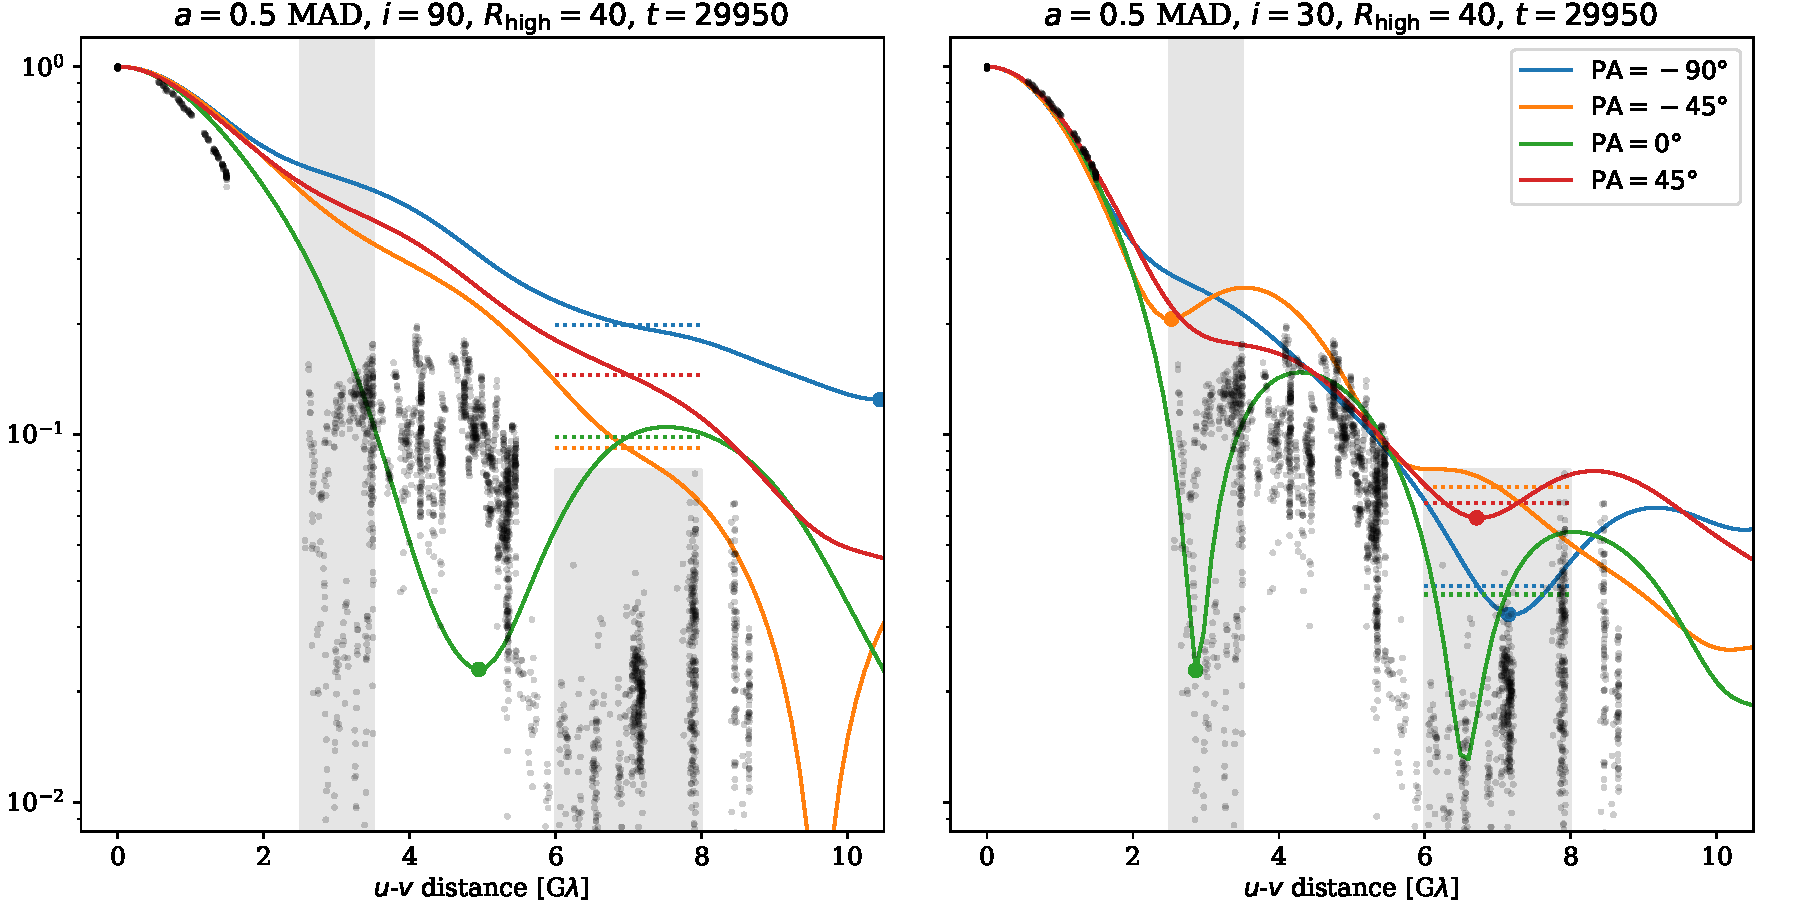
\includegraphics[width=0.75\textwidth]{figures/passfail_va.pdf}
  \caption{\vam constraint example.  Left: passing snapshot; right: failing snapshot.  The solid lines in each plot show visibility amplitudes on a section through the origin in the \uv domain, at four position angles (PAs), where $0\degree$ is parallel to the projected angular momentum vector of the accretion flow.
  Solid black points show data from \aprilvii.  The \vam constraint requires that for at least one PA the first minimum in VA fall within the left grey band, and for all PAs the median of the VAs lie inside the right grey band (see Section~\ref{sec:vam} for details).  Evidently the snapshot at right fails {\em both} conditions.
  }
  \label{fig:passfail_va}
\end{figure*}

\begin{figure*}
  \centering
  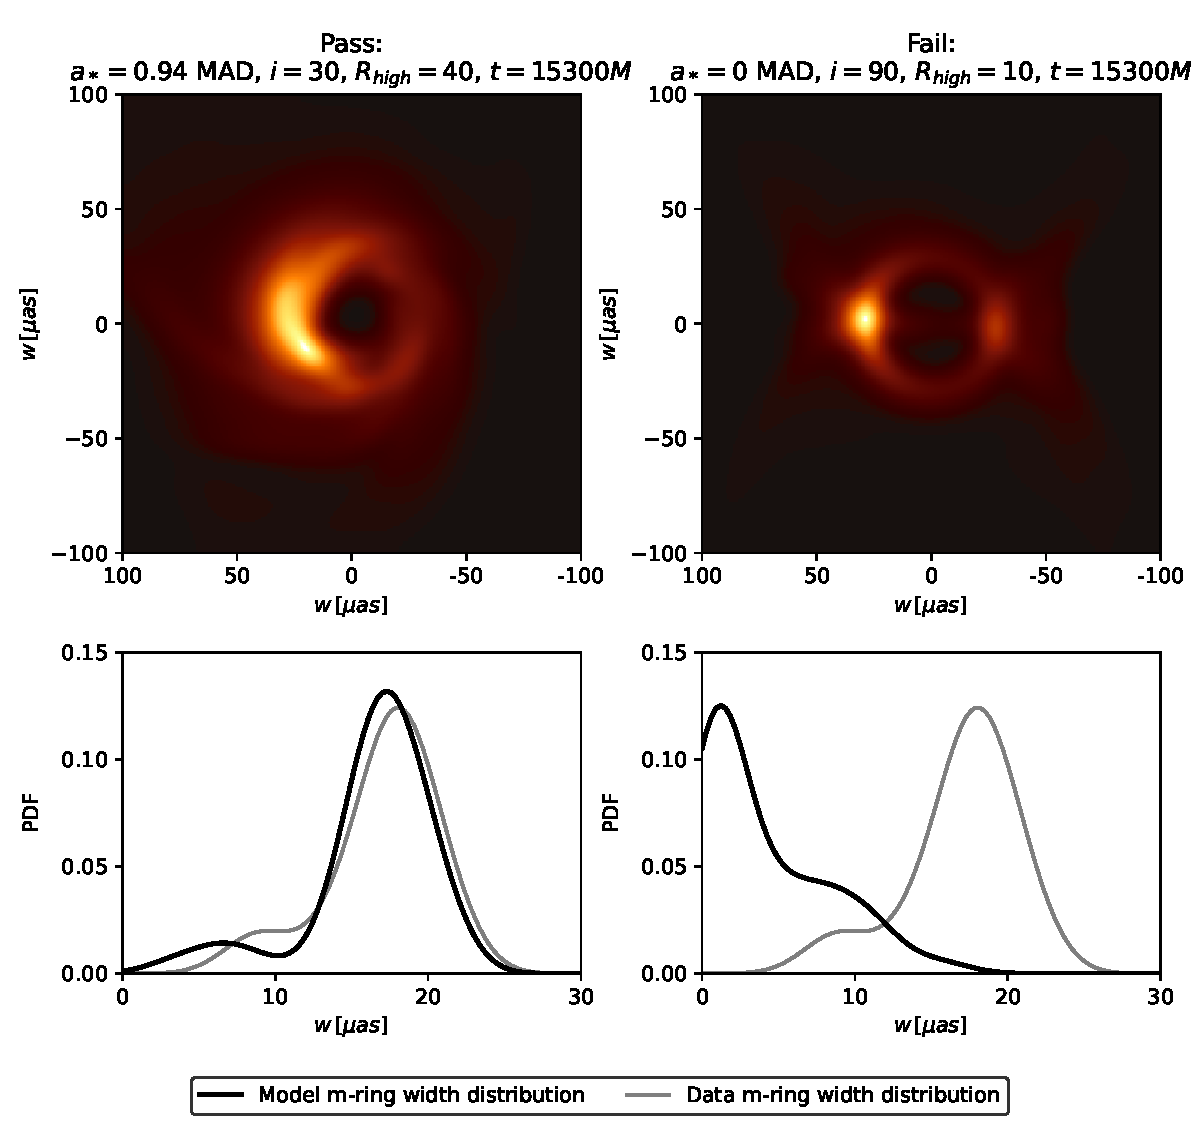
\includegraphics[width=0.75\textwidth]{figures/mring_width_example.pdf}
  \caption{\Mring width constraint example.  Top left: image that satisfies the constraint, Gaussian blurred to $20\uas$; top right: image that fails the constraint; bottom left: observed distribution of \mring widths over our 10 selected scans (light grey) and passing image distribution over 10 scans and 4 position angles (black); bottom right: observed distribution of \mring widths over our 10 selected scans (light grey) and failing image distribution (black) over 10 scans and 4 position angles.
  }
  \label{fig:mring_width_example}
\end{figure*}

The \vam constraint tests if the VAs of a model match the
observations by comparing its null location and long-baseline visibility
amplitude.  As Figure~\ref{fig:passfail_va} demonstrates, this constraint is
informative.  The constraint disfavors edge-on MAD models at positive spin and a few large $\Rh$ SANE models.  This is mainly because the edge-on MADs are bright blobs with faint rings, so the first nulls get washed out by the bright features.  The null location constraint rejects 16\% of \kharma models, 17\% of \bhac models, and 20\% of \hamr models.

%..............................................................................
\subsubsubsection{\Mring Fits}
\label{sec:mring}

The \mring asymmetry, diameter, and width fits are treated as separate constraints.  Recall that we compare the distribution from the data to that from the model use a two-sample KS test. 

The asymmetry parameter is typically not well constrained. Most rejected models are high inclination MAD models with $\abh \ge 0$.  Some of these models have asymmetries that are large and detectable because Doppler boosting concentrates emission in an equatorial spot on the approaching side of the disk.  The asymmetry parameter rejects 6\% of \kharma models, 5\% of \bhac models, and 1\% of \hamr models.  

The ring diameter is better constrained than the asymmetry parameter and varies systematically from model to model. For example, the distribution of diameters is much broader at $\Rh = 1$ than at larger values of $\Rh$.  More models therefore fail the ring diameter test, which rejects 33\% of \kharma models, 35\% of \bhac models, and 39\% of \hamr models.  

Most of the models that fail are low inclination models with ring diameters that are too large (no models fail because the ring diameter is too small).  For example, the $i = 10\degree$, $\Rh = 10$ SANE models fail for all spins with $\abh \le 0$ because the ring is too large.  The same is true for all $i = 10\degree$ MAD models with $\Rh = 1$.

% cfg 1/30: removing this claim because of questions raised in internal report
%Notice that the ring diameter is not degenerate with the second moment constraint; all models that fail the latter pass the former.  Recall that in addition to a blurred ring, the \mrings model contains a centered Gaussian component; the Gaussian tends to grow to absorb the emission when the ring is very extended.

The distribution of ring diameters for many SANE models is multimodal (consistently so in the fiducial model sets), with a secondary peak in the distribution at $\sim 35\uas$.  All $\Rh = 1$ SANE models show this secondary peak.  The images of these models tend to have a well defined ring at the critical impact parameter and a second broad maximum in intensity at larger impact parameter.  The second peak in the distribution is a consequence of limited baseline coverage.

The \mring width $w$ is the most tightly constrained of our 3 parameters. Although the closure phases constrain $w$ as well, it is easiest to see how $w$ affects visibility amplitudes at long baselines. For example, for a simple, symmetric ring the visibility amplitudes are a Bessel function multiplied by a Gaussian with width $\sim 1/w$, and increasing $w$ therefore decreases the amplitude of the long baselines.  Figure~\ref{fig:mring_width_example} shows examples of models that pass and fail the \mring width constraint. 

Figure~\ref{fig:mring_width_salsa} summarizes the \mring  pass/fail status of the fiducial models. All rejected models have median $w$ that is below the median of the data, $ \simeq 17.5\mu$as.  The rejected models include all but 3 MAD models at $\abh \le 0$ and all edge-on ($i = 90\degree$) MAD models in the  \kharma, \bhac, and \hamr fiducial models.  MAD models exhibit a strong trend toward smaller $w$ as $i$ increases.  SANE models exhibit a similar but weaker trend. The SANE model images have  higher optical depth, broader rings, and more substructure than the MAD models.  Their $w$ distributions are typically broad, with mode well below $17.5\mu$as.  Only for $\abh = 0.94$, where the optical depth is lower due to higher temperatures in the emitting region, do most of the models exhibit a sharply peaked $w$ distribution centered at $17.5\mu$as.

\begin{figure*}\label{fig:mring_width_salsa}
 \centering
 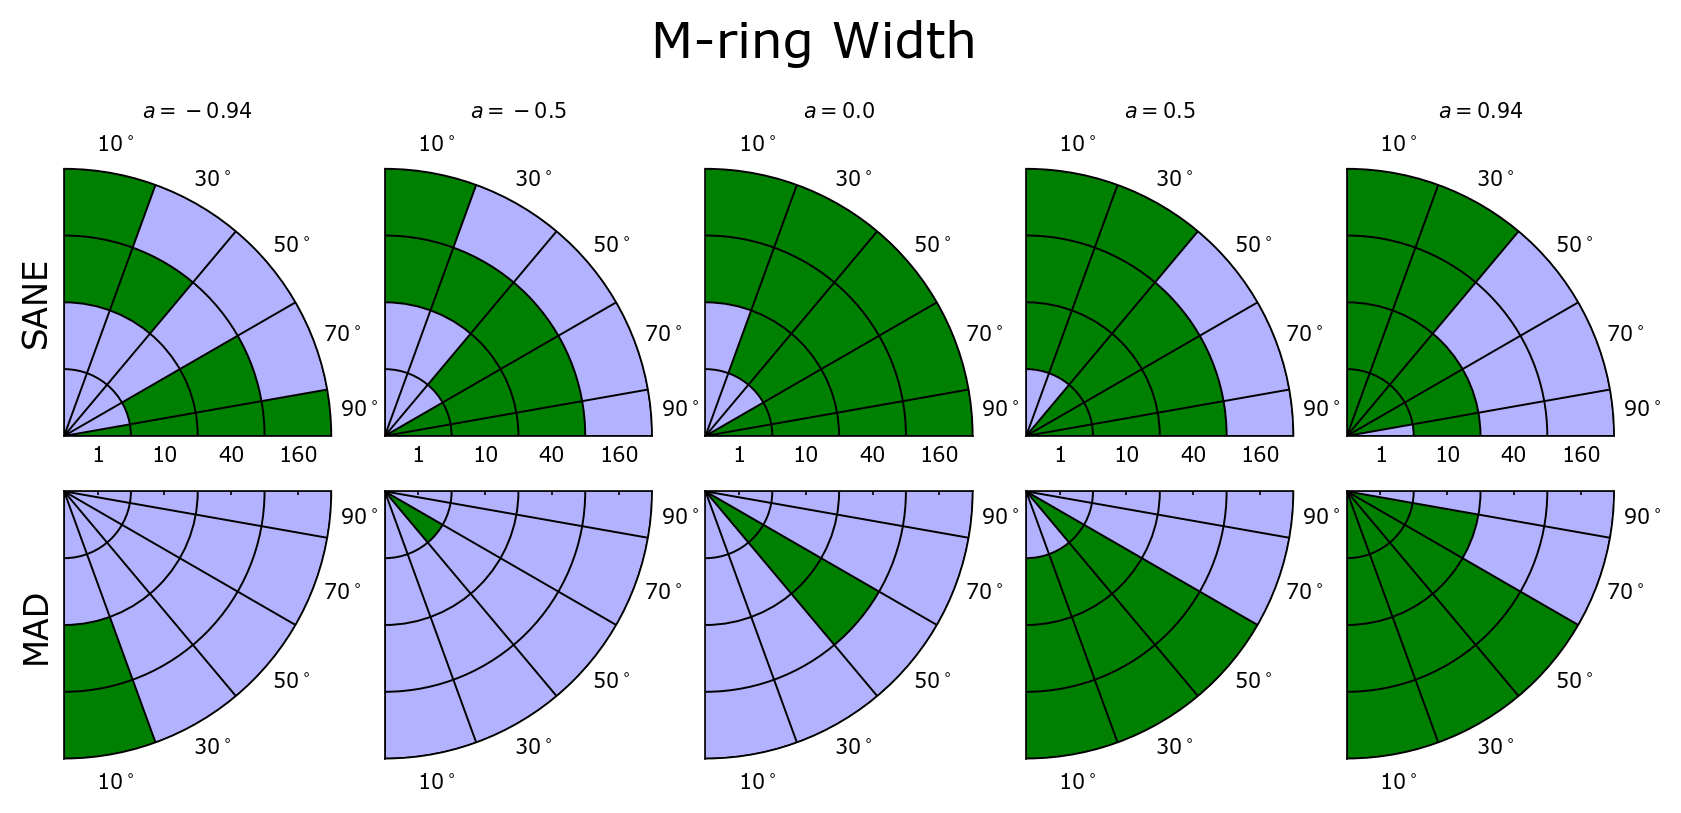
\includegraphics[width=\textwidth]{./figures/Mring_w_Constraints.png}
  \caption{Pass/fail plot for the \mring widths.  Green indicates that the \kharma, \bhac, and \hamr models pass, yellow that one or two of the fiducial models fail, and red that all three fail.  The inclination coverage is not uniform: \bhac and \kharma models cover all 5 inclinations while \hamr models cover $i = 10, 50, 90$ only.  The $i = 30, 70$ wedges therefore include only the \bhac and \kharma models.}
\end{figure*}


\subsubsubsection{EHT Constraint Summary}

We can combine all EHT constraint cuts with a logical {\em and} operation.  The results are summarized in Figure~\ref{fig:all_EHT_constraints}.  Evidently EHT data alone are capable of discriminating between models.   The edge-on ($i = 90\degree$) models all fail, with some failing \mring width, diameter, asymmetry and the null location constraint.  The cuts clearly favor $\abh > 0$ models, with a few exceptions.  There are two clusters of models that do not fail any constraints in any models: positive spin MAD models at low inclination, and positive spin SANE models, also at low inclination.   

\begin{figure*}\label{fig:all_EHT_constraints}
  \centering
    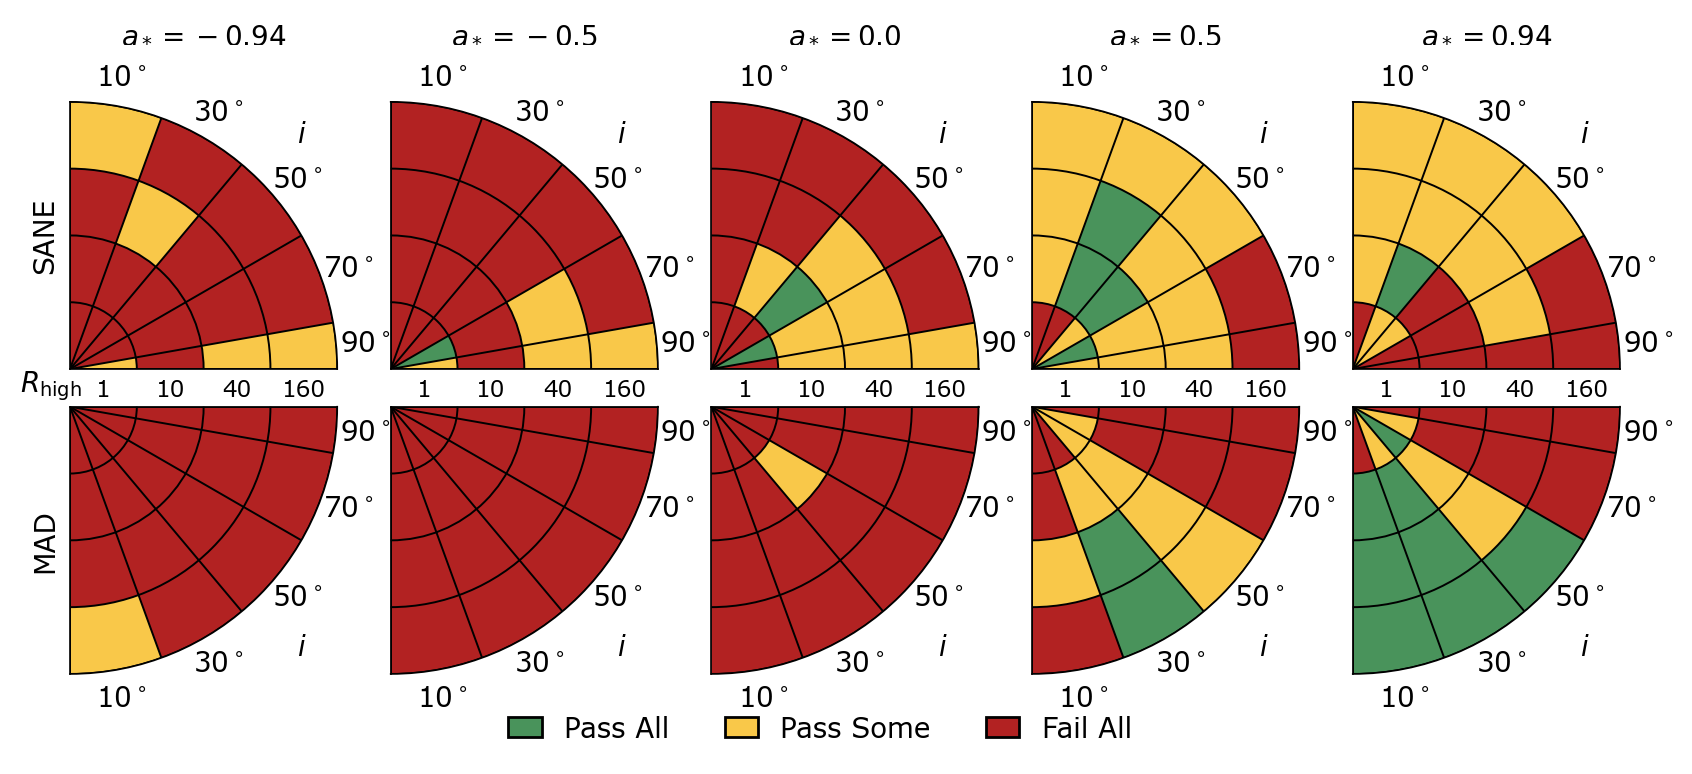
\includegraphics[width=\textwidth]{./figures/Interferometric_Constraints.png}
  \caption{Combined EHT constraints (logical {\em and}) including the second moment, null location, and \mring fit constraints.  Green indicates that the \kharma, \bhac, and \hamr models pass, yellow that one or two of the fiducial models fail, and red that all three fail.  The inclination coverage is not uniform: \bhac and \kharma models cover all 5 inclinations while \hamr models cover $i = 10, 50, 90$ only.}
\end{figure*}

\subsubsection{Non-EHT Constraints}

We now consider constraints from unresolved $86\GHz$, $2.2\um$, and X-ray
observations.
Some or all of the emission in these bands are believed to originate
in the compact source from plasma that is close to or overlaps the
plasma that is producing the 230\GHz-emitting plasma observed by EHT.
Figure~\ref{fig:noneht_pizza} shows which models pass and fail these
constraints in aggregate.

\begin{figure*}
  \centering
  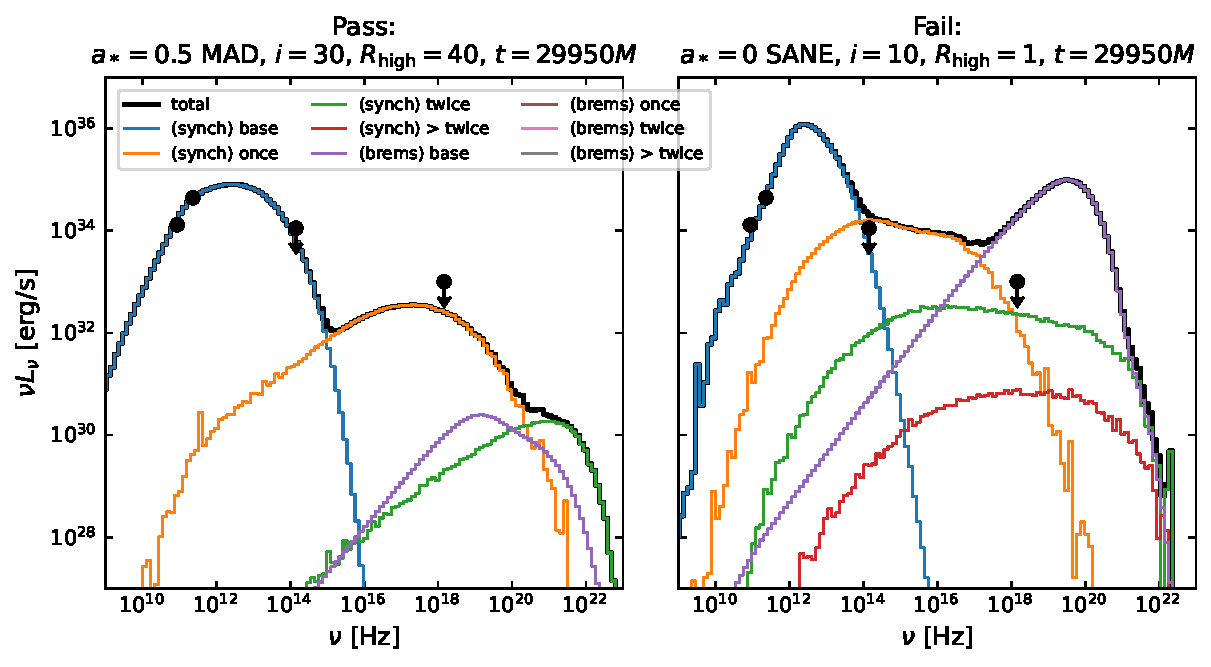
\includegraphics[width=0.9\textwidth]{figures/passfail_sed.pdf}
  \caption{
    Non-EHT flux density constraint example.  Left: passing model with SED close to the measured 86\GHz point and below the quiescent $2.2\um$ and X-ray points.  Right: failing model with inconsistent (strongly rising) millimeter wavelength spectral index, overproduction of $2.2\um$ due to strong Comptonization, and overproduction of X-rays by bremsstrahlung.
    }
  \label{fig:passfail_sed}
\end{figure*}

\subsubsubsection{86\GHz Median Flux}

In a naive picture \sgra's millimeter flux is produced in a photosphere that decreases in size as frequency increases.  Because optical depth is not large at 230\GHz ($\sim 0.3$ in the one-zone model) and the source structure is complicated (the optical depth varies across the image) the naive picture is imprecise.  Nevertheless 86\GHz photons are on average produced at larger radius than 230\GHz photons, and the 86\GHz source size is larger than the 230\GHz source size.

The ratio of 86\GHz to 230\GHz flux density is therefore sensitive to the radial structure of the source plasma.  Figure \ref{fig:86GHz_flux_pizza} shows the full results of applying this constraint.
%\cfg{need more physical discussion}
Many $\Rh = 1$ models, both MAD and SANE, fail the 86\GHz flux density test. $76\%$ of SANE models and $24\%$ of MAD models overproduce 86\GHz emission in all three fiducial model sets.%A large set of SANE models (17/100) underproduce 86\GHz emission, and these have $10 \le \Rh \le 40$
The 86\GHz flux is sensitive to $\Rh$.  For example, SANE $\abh = 0.5$, $i = 70,90$deg models are too bright at $\Rh = 1$ and too dim at $\Rh = 10$.  There must be passing models in between, suggesting our parameter space is not sampled densely enough.

%..............................................................................
\subsubsubsection{86\GHz Major Axis}

Similarly to the 86\GHz flux, the 86\GHz size is sensitive to optical depth as a function of radius in the source plasma. Figure~\ref{fig:86GHz_size_pizza} in Appendix~\ref{app:tables} shows the full results of applying this constraint.

%\cfg{need cites to earlier work for par below}

The 86\GHz size is sensitive to inclination.  For example, the SANE, $\abh = 0$, $\Rh = 40$ models are too small at low inclination and too large when seen edge-on, because the edge-on models have prominent limb-brightened jet walls that are visible to 100$\mu$as.  The 86\GHz size constraint rejects
$42\%$ of models and is therefore one of the tightest constraints.

The physical picture for 86\GHz source size is complicated, as is the extraction of the constraint itself from observations.  Notice that (1) two different values for the 86\GHz intrinsic source size have been reported in the literature (see Section \ref{sec:86size}); (2) scattering is $7$ times stronger at 86\GHz than at 230\GHz; (3) scattering must be subtracted accurately to obtain the intrinsic source size; (4) the error bars for the 86\GHz source size are narrow and this plays a key role in determining the strength of the constraint.

\subsubsubsection{$2.2\um$ Median Flux Density}

$2.2\um$ photons are produced by the synchrotron process from electrons on the high energy end of the eDF.  For the one-zone model with $B = 30$G and $\Theta_e = 10$ the mean Lorentz factor is $\gamma = 30$ and the synchrotron critical frequency $\nu_\mathrm{crit} = \gamma^2 e B/(2 \pi m_e c) \simeq 80\GHz$.  Emission at $2.2\um$ is therefore produced by electrons with  Lorentz factor $\gamma \simeq 10^3$, so $2.2\um$ flux density is sensitive to $\Theta_e$ and $B$.  Since both increase toward the horizon and field strength is nearly independent of latitude, $2.2\um$ photons are produced at small radius in regions where $\Theta_e$ is highest.

The sensitivity to $\Theta_e$ implies that $2.2\um$ flux density will be highest for parameters with higher temperatures.  For SANEs the midplane temperature increases with $\abh$.
The sensitivity to $B$ implies that $2.2\um$ flux density will be highest for parameters with stronger fields.  The $B$ depends on the GRMHD flow configuration and also on the accretion rate, which is fixed by the observed $F_{230}$, so $2.2\um$ will be strongest when the accretion rate is largest.  For SANEs, accretion rate declines as $\abh$ increases and $\Rh$ decreases (discussed in more detail below in  Section~\ref{sec:accrate_outflowpower} and Figure \ref{fig:accretion_outflow_power_illinois_thermal}); for MADs the accretion rate dependence on $\abh$ and $\Rh$ is much weaker.
Finally, the Doppler effect (blueshift) enables photons that are detected at $2.2\mu$m to be emitted at longer wavelength in plasma that is moving toward the observer, and the accompanying Doppler beaming increases the detected intensity.  We therefore expect $2.2\um$ flux density to increase with inclination and to peak in the midplane on the approaching side of the flow.

Models that pass the $2.2\um$ flux limit are shown in the Appendix in Figure~\ref{fig:2um_flux_pizza}. The rejected SANE models ($7\%$) tend to be at positive spin and high inclination: their images are dominated by a bright spot on the approaching side of the disk.
The rejected MAD models ($53\%$) include all but 4 models at $\Rh = 1$ and all but 2 models at $\Rh = 10$, where $\Theta_e$ tends to be larger, and the majority of high-inclination models, where the effect of Doppler boosting is largest.

Interestingly, we find that some models are Compton dominated at $2.2\um$.  For example, $\abh = -0.94$ SANE models become optically thin at relatively low frequency as $\Rh$ goes to $1$, and thus synchrotron emission drops off rapidly as frequency increases.
As $\Rh$ drops and synchrotron decreases the SED becomes dominated by a lower-luminosity bump of underlying Comptonized photons.  Just before this happens, at $\Rh = 10$, the combination of the Compton bump and synchrotron emission is enough to push the median $2.2\um$ flux density above the observational limit, explaining the excluded SANE models at $\Rh = 10$, $\abh = -0.94$.


\subsubsubsection{X-ray Luminosity}

Many thermal models produce X-ray emission through Compton upscattering of thermal synchrotron photons.  In the first Compton bump $\nu L_\nu$ is proportional to the y-parameter $y \sim 16 \Theta_e^2 \tau_e$ where $\tau_e$ is a characteristic electron-scattering optical depth and $\Theta_e$ is a typical electron temperature.  At $\Rh = 1$ the X-ray band lies in the first Compton bump, while at larger $\Rh$ the bumps move to lower energy because the bulk of the Thomson depth is in the midplane where $\Theta_e \propto 1/\Rh$.

In many large $\Rh$ SANE models, however, X-ray emission is dominated by bremsstrahlung.  Since its emissivity $j_{\nu,b} \propto n^2$, bremsstrahlung is dominated by regions with the highest density, i.e., the midplane.  It typically comes from larger radius than the synchrotron and Compton-upscattered X-ray emission and therefore varies more slowly.  Bremsstrahlung therefore dominates Compton in the highest accretion rate models, i.e. when $\Rh$ is large (see Section~\ref{sec:discussions}).  Notice that $j_{\nu,b} \propto \Theta_e^{1/2}$ for $\Theta_e > 1$ and $\Theta_e^{-1/2}$ for $\Theta_e < 1$, so cool disks enhance bremsstrahlung.

The X-ray cut results are shown in Appendix~\ref{app:tables} in Figure~\ref{fig:xray_pizza}. Most large $\Rh$ SANE models fail the X-ray test: all but 2/25 at $\Rh = 160$ and all but 2/25 at $\Rh = 40$.  These models fail due to excess bremsstrahlung. The MAD models that fail have low $\Rh$ and are Compton-dominated in the X-ray.  All but one $\Rh = 1$ MAD models fail the X-ray test, as do approximately half at $\Rh = 10$.  The midplane $\Theta_e$ declines as $\Rh$ drops.  Since the midplane contributes most of the electron scattering optical depth, low $\Rh$ models have the largest $y$ parameter and are at greatest risk of overproducing X-rays. \michi{Need to update this explanation to reflect contradicting \bhac results}

\subsubsubsection{Summary of Non-EHT constraints}

Applying only non-EHT constraints, we are left with the $7\%$ of models shown in Figure~\ref{fig:non_eht_cuts}. The surviving models are the result of applying a heterogeneous and noisy set of constraints using a hard cutoff, which obscures the underlying physical picture.  Nevertheless, the surviving models are all MAD, all have $\Rh > 10$, and all but two are at $i < 70\degree$.  This leaves a cluster of surviving MAD models at large $\Rh$ and moderate inclination.

\begin{figure*}\label{fig:non_eht_cuts}
  \centering
  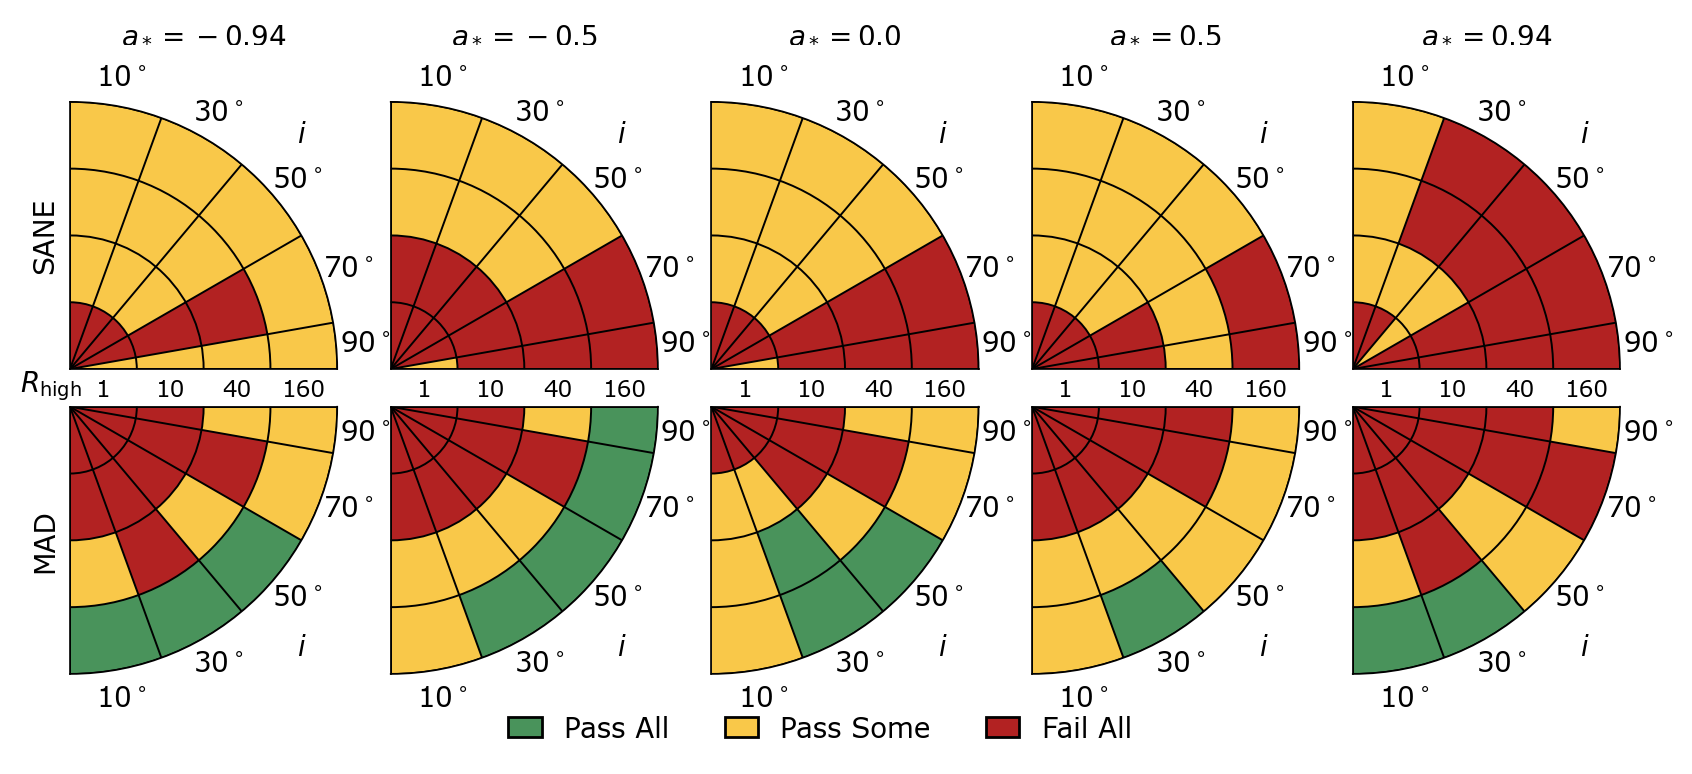
\includegraphics[width=\textwidth]{./figures/Non_Interferometric_Constraints.png}
  \caption{Combined non-EHT constraints (logical {\em and}).  Green indicates that the \kharma, \bhac, and \hamr models pass, yellow that one or two of the fiducial models fail, and red that all three fail.}
\end{figure*}

%------------------------------------------------------------------------------
\subsubsection{Variability}

Variability is central to  the interpretation of \sgra: an $8\,\mathrm{hr}$ observation of \sgra is $1400 \tg$, a timescale over which most models vary substantially.  In contrast, an $8\,\mathrm{hr}$ observation of M87* is $\sim \tg$ and on this timescale M87* and \sgra hardly vary at all.
%\footnote{This does not mean that \m87 is less variable than \sgra, just that we do not have }

Variability is a strong constraint.  Although models differ in their degree of variability, both in an integrated sense and on 2--6~$G\lambda$ baselines, only a small fraction of models are as quiet as the data.  For the lightcurve variability, this remains true whether we use data from April 7, 2017, all days from the 2017 observing campaign, or from historical monitoring of \sgra.   In general, we find that SANE models are quieter than MAD models, and (to a lesser extent) face-on models are quieter than edge-on models.

If we were to apply the variability constraints directly to the models, there would be 37/200 successful models remaining using 1\% cuts (47/200 for the ALMA constraint and 121/200 for the visibility amplitude constraint).  One interpretation of this result is that the surviving models are the correct description of the source (although we would expect some misclassification of models as consistent or inconsistent when using 1\% cuts on such a large model set).  Another interpretation is that there is a missing physical ingredient in the models, which could affect our entire model library. This possibility is discussed in Section \ref{sec:discussions}.

%..............................................................................
\subsubsubsection{Modulation Index}

The distributions of 3 hour modulation index ($\mi{3}$) across all fiducial SANE models, across all fiducial MAD models, and across the historical dataset are shown in Figure \ref{fig:cmp_ALMA_var}.  The plot also shows individual distributions for models with the lowest and highest $\mi{3}$.  

The full set of fiducial model results from the $\mi{3}$ constraint is shown in Appendix \ref{app:tables}, Figure \ref{fig:m3_pizza}.  
We find that: (1) as a group, the fiducial models are more variable than the data; (2) the MAD models are more variable than SANE models; (3) eleven individual models  pass the constraint for all fiducial model sets, and these are exclusively SANE models; (4) there are some differences between variability in the fiducial model sets, with \hamr models notably more variable than \kharma and \bhac models; (5) the pass fractions for the fiducial model sets are $0.2$ for \kharma, $0.27$ for \bhac, and $0.07$ for \hamr.   The modulation index is, by far, the tightest single constraint on the models.  

\begin{figure}
  \centering
  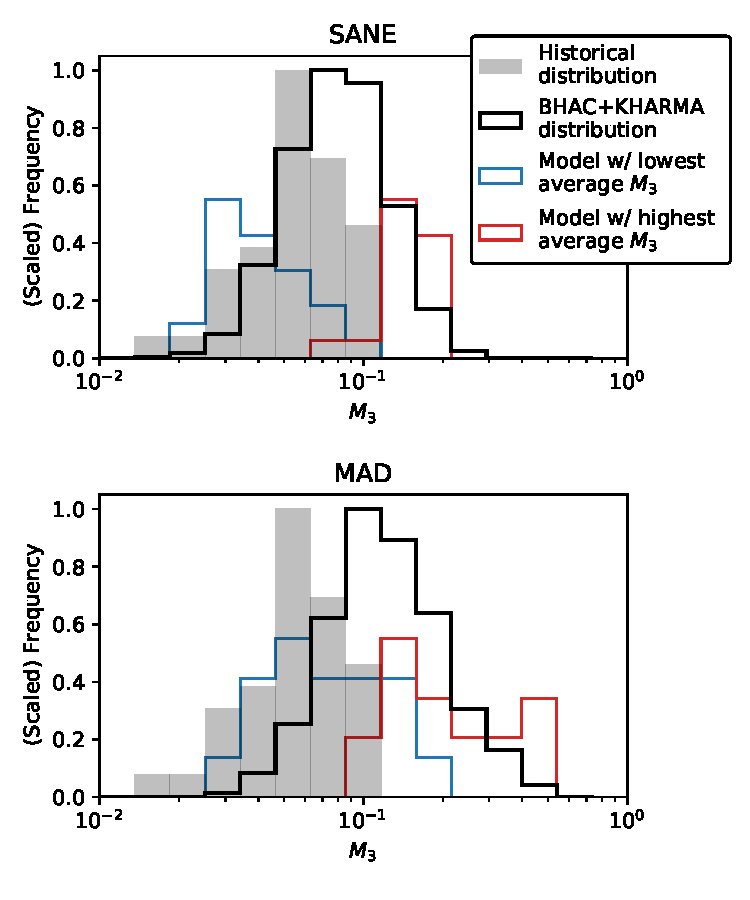
\includegraphics[width=\columnwidth]{./figures/mi_hist.pdf}
  \caption{Distributions of 3-hour modulate index $\mi{3}$ for \bhac, \kharma, and \hamr models (black), compared to distributions from historical observations (gray). The distributions for models with the lowest (blue) and highest (red) average $\mi{3}$ for SANEs and MADs are also shown. The heights of these distributions have been scaled for clarity.
  }
  \label{fig:cmp_ALMA_var}
\end{figure}

%..............................................................................
\subsubsubsection{4 \texorpdfstring{$G\lambda$}{Gl} Visibility Amplitude Variability}

The power-law index $b$ of the variance $\sigma_\text{var}^2 (|u|)$ at 2--6$~{\rm G}\lambda$ of the models is generally in good agreement with the value measured  from the 2017 EHT campaign (excluding April 11). The amplitude $\afour^2$, however, varies depending on the model.

Figure~\ref{fig:cmp_VLBI_var} shows the distribution of $(\afour^2, b)$ from the EHT observation, along with the distributions across all fiducial models. For a single model, the number of measurements of $(\afour^2, b)$ is equal to the number of windows for that model (three in most cases). 

%The models are shown together, but each model consists of only three measurements of $\afour^2$, one on each window of length $5 \times 10^3 \tg$. This makes a direct comparison with the measured value difficult, as the distribution for a given model is poorly constrained.

%\citet{Georgiev_2022} gives an estimate of the typical width of the distribution as $\log_{10}(\afour^2) \pm 0.1$. We can obtain a rough estimate for how the models fare compared to the measurement by taking the mean across windows and the estimate for the width and comparing this with the measurement distribution under the assumption that both are distributed normally. With this approach, 121/200 models (63 SANE and 58 MAD) agree with the data within 1\%, although we caution against interpreting this number as the number of passing or failing models, since the uncertainties in the model distribution are so large.

The models tend to be slightly more variable than the observation, with face-on models performing better than edge-on models. For SANE models, $\Rh = 10$ tend to be more variable than others. For MAD models, there is a slight preference for lower $\Rh$.

We have also considered a set of thermal, $\Rh$, MAD models run with the \koral code out to $\sim 100,000\tg$.  These models enable us to assess the importance of integration time for application of the constraints.  They permit us to obtain more accurate distributions for the constraint quantities and to assess whether the constraints evolve from the beginning to end of the integrations. We do not see evidence for evolution in the \koral model set (a full pass/fail table is given in Appendix~\ref{app:tables}, Table~\ref{tab:koralPF} and more detailed discussion in Appendix~\ref{app:variability} and in \citet{Georgiev_2022}). The \koral pass/fail results are similar to those for comparable models in the fiducial model sets. Moreover the constraints measured at the beginning of the evolution are similar to those measured at the end.

\begin{figure}
  \centering
  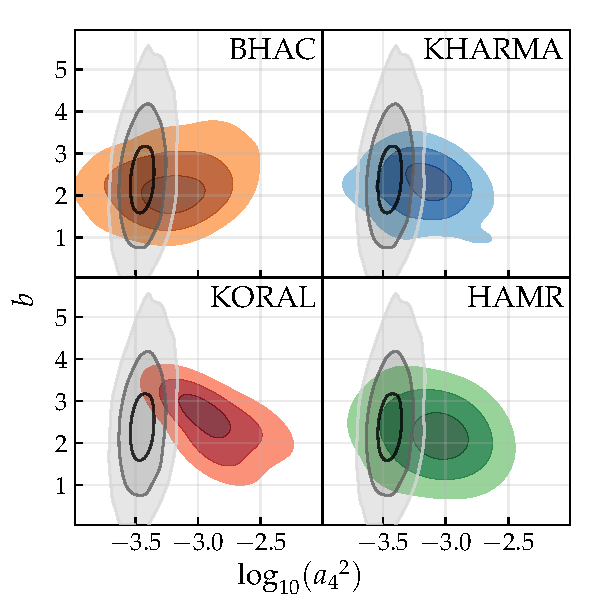
\includegraphics[width=\columnwidth]{./figures/grmhd_triangle_debiased_combined.pdf}
  \caption{Distributions of $(\log_{10}(\afour^2),b)$ for \bhac, \kharma, \koral, and \hamr, compared against the 2017 EHT confidence regions (gray). }
  \label{fig:cmp_VLBI_var}
\end{figure}

% At a 1\% cut, the models that pass the PSD constraint also all pass the MI constraint. It should be noted that this is partially because these constraints are weakly correlated \dl{also partially because we're imposing constraints differently between VLBI and lightcurve, and the lightcurve constraint is more lenient} None of the 12 models with acceptable variability pass the other tests.

%------------------------------------------------------------------------------
\subsubsection{Summary of Constraints on Fiducial Models}

\begin{deluxetable*}{l|ccccc}\label{tab:fail_one_thermal}
\tablecaption{Fiducial models that fail only one constraint}
\tablehead{
\colhead{Code/Setup} &
\colhead{MAD/SANE} &
\colhead{Spin $\abh$} &
\colhead{Inclination $i$} &
\colhead{$\Rh$} &
\colhead{Failed Constraint}
}
\startdata
\kharma Thermal					&	SANE	&	0.94	&	10		&	40		&	86\,GHz size		\\
\kharma Thermal					&	SANE	&	0.94	&	30		&	40		&	86\,GHz size		\\
\kharma Thermal					&	SANE	&	0.94	&	50		&	1		&	86\,GHz size		\\
\kharma Thermal					&	MAD		&	0.5		&	30		&	40		&	\mi{3}				\\
\kharma Thermal					&	MAD		&	0.5		&	30		&	160		&	\mi{3}				\\
\kharma Thermal					&	MAD		&	0.94	&	10		&	160		&	\mi{3}				\\
\kharma Thermal					&	MAD		&	0.94	&	30		&	160		&	\mi{3}				\\
\hline
\bhac Thermal					&	SANE	&	-0.5	&	30		&	40		&	\Mring diameter   	\\
\bhac Thermal					&	SANE	&	0		&	30		&	40		&	\Mring diameter   	\\
\bhac Thermal					&	SANE	&	0.5		&	10		&	40		&   \mi{3}  			\\
\bhac Thermal					&	SANE	&	0.5		&	10		&	160		&   \mi{3}  			\\
\bhac Thermal					&	SANE	&	0.5		&	30		&	40		&   \mi{3}  			\\
\bhac Thermal					&	SANE	&	0.5		&	30		&	160		&   \mi{3}  			\\
\bhac Thermal					&	MAD		&	0.5		&	30		&	160		&   \mi{3}  			\\
\bhac Thermal					&	MAD		&	0.5		&	50		&	160		&   \mi{3}  			\\
\bhac Thermal					&	MAD		&	0.94	&	10		&	160		&   \mi{3}  			\\
\bhac Thermal					&	MAD		&	0.94	&	30		&	160		&   \mi{3}  			\\
\enddata
\tablecomments{Models which pass all of the constraints except for one. Since no model passes all constraints, these represent the parameters that are closest to being consistent with observations.}

\end{deluxetable*}


\label{sec:summarythermal}

None of the fiducial models  survive the full gauntlet of constraints.   The pass fractions for individual constraints for the \bhac, \kharma, and \hamr fiducial models are listed in Table \ref{tab:passfraction_thermal}.  Notice that the variability constraint is the most severe, followed by the \mring width constraint.  Variability rejects about $80\%$ of fiducial models and prefers SANEs, which are quieter than MADs, while the remaining constraints prefer MAD models.

It is possible (even likely) that the models are physically inadequate.  But it is also possible that one of the constraints is measured incorrectly, that one of the constraints is applied incorrectly, or that one of the constraints is poorly predicted for numerical reasons.  To investigate this, we identify all models that fail only one constraint in Table \ref{tab:fail_one_thermal}.  The critical constraints are 86\GHz size, \mring diameter, and $\mi{3}$.  Notice that there is overlap between \kharma and \bhac in MAD models that fail the $\mi{3}$ constraint.  No \hamr models are listed because all \hamr models fail at least two constraints.    

% CFG: commented out 1/31.  This material should go in the discussion section

%Evidently either (1) the models fail in some important respect, or (2) some of the data underlying the model tests are incorrect, or (3) one or more of the constraints have been misapplied.  We 

%We will discuss option (1) later.  To investigate options (2) and (3), we can ask what happens when we lift one constraint.  Table~\ref{tab:fail_one} lists the models that fail only one constraints---about 5\% each for the \bhac and \kharma model sets.  For \bhac, 8 models fail only $\mi{3}$, and 2 fail only \mring diameter.  For \kharma, 3 models fail only $\mi{3}$ and 5 fail only the 86\GHz size.  Suspicion therefore falls on $\mi{3}$, which rejects $\approx 70\%$ of \bhac and \kharma models.  Why might the $\mi{3}$ constraint be misleading?

%One possibility is that some fraction of the $230\GHz$ flux density, $f_\mathrm{ext}$, is in an extended structure (a jet) that is slowly varying, captured in the ALMA lightcurves, and resolved out by EHT.  The implied $f_{ext}$ is model-dependent, but if $f_{ext} \sim 30\%$ then nearly all MAD models would pass $\mi{3}$ and many SANE models would be rejected as too quiet.  The $4$G$\lambda$ amplitude variability is normalized by the lightcurve and thus $a_4$ would increase by a similar factor.  Notice that if $f_{ext} > 0$ then the models would need to be re-normalized (the accretion rate adjusted) so that the compact flux is $(1 - f_{ext}) \times 2.4\,\mathrm{Jy}$.  The extended flux hypothesis can be tested by the addition of new, short baselines to the EHT.

%A second possibility is that physical or numerical errors in the models cause the variability to be overstated.  Several possibilities, including viscosity, conduction, and radiative cooling are discussed in Section \ref{sec:discussions}.

%If extended flux, viscosity and conduction, and radiative cooling each reduce the variability excess by $\sim 10\%$ then many of the MAD models would come into compliance with the data (and some SANE models would become inconsistent because they are not variable enough).  If we set aside the $\mi{3}$ constraint then a cluster of 3 models survives all of the fiducial models.  All are MAD, $\Rh = 160$.  These are: $\abh = 0.5, i = 30$; $\abh = 0.94, i = 10$; and $\abh = 0.94, i = 30$.  These models are clustered in parameter space and pass 10 of 11 tests.  We will highlight these models below in our discussion and analysis.

%We consider exploratory models next, including nonthermal eDF models, wind-fed models, and tilted models.  None have sharply reduced $\mi{3}$.


\subsection{Exploratory Models}\label{sec:explore}

Next we go beyond the fiducial aligned, thermal, $\Rh$ models and consider aligned models that use an alternative scheme for assigning temperatures to a thermal eDF; aligned models with a power-law component or $\kappa$ component in the eDF; tilted models; and stellar wind-fed models.  Unless stated otherwise, exploratory models are imaged over only $5 \times 10^3 \tg$, yielding weaker constraints on the models.

%------------------------------------------------------------------------------
\subsubsection{Critical Beta Model}

The fiducial $\Rh$ prescription provide a convenient, one-parameter model for assigning electron temperatures, but here is a vast function space of possible alternative parameterizations. One well-motivated choice is the critical beta model \citep{2020MNRAS.493.1404A}, which sets $T_e = T_e(R)$ and $R = f \exp(-\beta/\beta_c)$ (see Equation \ref{eq:thermaleDF}).  This ``critical beta'' model has two parameters, $f$ and $\beta_c$.  We consider a single point in the parameter space: $f = 0.5$, $\beta_c = 1$.  Compared to the \Rh temperature prescription, the main new characteristic of the critical beta models is that the electron to ion temperature ratio approaches 0 at high $\beta$ instead of $1/\Rh$, allowing much lower electron temperatures at high $\beta$.

We have run all tests except X-ray for the critical beta models. $2.2\um$ is calculated with imaging only and therefore does not include Compton scattering.  

%The full set of results is given in Appendix~\ref{app:tables}, Table~\ref{tab:betacritPF}.

All critical beta models fail the non-EHT constraints, with the 86GHz size constraint rejecting most models as too small.  The variability constraints fail $77\%$ of the models.  No models survive the combined EHT and non-EHT constraints, excluding variability.  Notice that this does not imply that critical beta models are ruled out, since we have only tested a single parameter set.

\subsubsection{Thermal Plus \texorpdfstring{$p = 4$}{p=4} Power-law Models}

So far we have assumed a thermal relativistic Maxwell-J{\"u}ttner eDF (Equation~\ref{eq:thermaleDF}). Fully kinetic simulations as well as resistive MHD predict that reconnection in current sheets within the accretion flow and in the jet sheath leads to the acceleration of particles to higher energies, resulting in the emergence of a power-law tail (of the form of Equation~\ref{eq:nonthermaleDF}) in the eDF \citep[e.g.,][and references therein]{Sironi2021}. Such acceleration events are thought to be the origin of near-infrared and X-ray flares detected in \sgra. In this work, we do not address flare mechanisms but seek to constrain the contribution of non-thermal electrons to the quiescent emission of \sgra. 

In the next few sections, we assume different forms of the eDF assuming that a fraction of the electron population is accelerated to a non-thermal tail. There are multiple ways of doing this, but we will continue to assume that the eDF depends instantaneously on local conditions and set the accretion rate so that the time-averaged 230\GHz compact flux is 2.4 Jy.

First we employ a hybrid thermal/power-law tail distribution using \hamr/\bhoss. Since we are modeling the quiescent emission of \sgra, we assume a steep power-law index of $p=4$ with a constant non-thermal acceleration efficiency $\epsilon=n_{\rm e, power-law}/n_{\rm e, thermal}=0.1$, typically found from PIC simulations \citep[e.g.,][]{Sironi2015,Crumley2019}. Following the method given in \citet{Chatterjee2021}, the power-law tail is stitched to the thermal core by choosing the minimum Lorentz factor limit of the power-law $\gamma_{\rm min}$ to be at the peak of the Maxwellian component. The upper end of the power-law is taken to $10^5 \gamma_{\rm min}$ (see Equation \ref{eq:nonthermaleDF}).  The temperature of the thermal component is set by the $\Rh$ prescription (Equation~(\ref{eq:rhigh_prescription})). We find that the accretion rate is slightly smaller than for corresponding thermal models, suggesting that the power-law component contributes to the 230\GHz total intensity. 
%The full pass/fail table of hybrid thermal/power-law models is given in Table~\ref{tab:hamr_nth}

%..............................................................................
\subsubsubsection{230\GHz VLBI pre-image size}

Hybrid thermal/power-law models have larger 230\GHz VLBI pre-image sizes compared to their purely thermal counterparts. This is because the power-law component of the eDF allows high energy electrons at distances more than a few gravitational radii (i.e., larger than the typical emission radius of the 230\GHz images.) to contribute to the total image. However, the extension in the images is much smaller for MAD models, with most images displaying a net increase in size of $<10\%$.

%..............................................................................
\subsubsubsection{86\GHz flux and image size}

In general the $R_{\rm high}=1$ models produce too much 86\GHz flux. Since the lower limit of the power-law $\gamma_{\rm min}$ is directly affected by the local electron temperature, the highest energy electrons are located in the jet sheath where the ion and electron temperatures are similar, i.e., $T_i\approx T_e$. Indeed this is why SANE models produce more 86\GHz flux when non-thermal electrons are introduced, especially at larger $R_{\rm high}$ values. On the other hand, MAD pure thermal and mixed thermal/non-thermal models behave similarly as the bulk of the emission is produced in the inner disk.

Due to the additional power-law component, the 86\GHz image sizes for the hybrid \hamr models are, on average, larger than their thermal-only counterparts, similar to the 230\GHz results. The higher energy electrons of a hybrid thermal/power-law population emit at higher frequencies than their thermal core, thereby extending the image size. This effect is not substantial in the case of MAD accretion models as the image sizes increase by a few percent only.

\subsubsubsection{$2.2\um$ constraint}

The addition of the power-law tail primarily increases the flux at $2.2\um$ and thus, the GRAVITY $2.2\um$ flux density of $1.0\,\mathrm{mJy}$ could provide a constraint on the power-law index and the acceleration efficiency. In brief, $\Rh=1$ and $40$ MAD models are ruled out by the $2.2\um$ constraint.

\subsubsubsection{Summary}

Overall, \hamr nonthermal powerlaw models behave quite differently from their thermal versions. For the thermal models, the non-EHT constraints prove to be more crucial in ruling out models (with 9/90 passed cases in total) while the EHT constraints were more lenient with 35/90 models passing. For the power-law model set, we get the opposite: non-EHT constraints pass 35/90 models while EHT constraints allow 10/90 models. This disparity occurs for two reasons: 1. Introducing non-thermal electrons pushes the 86 GHz image size to the acceptable range as thermal models typically exhibit small image sizes, and 2. the m-ring width is found to be smaller for the hybrid models. This could be due to a change in the gas density scaling that is required to match the 230GHz flux. Nonthermal models require a smaller normalization value, meaning a smaller electron number density as compared to the corresponding thermal models. A decrease in the number density would lower the optical depth as well, which could lead to a thinner photon ring. Ultimately, the number of passing models do not change (3 for thermal and 4 for nonthermal models), but the passing models are different: 2 SANE edge-on models from the thermal set and 2 MAD spin 0.5 Rhigh 1 models from the nonthermal set. Additionally, the $\mi{3}$ variability does not change when adding a power-law component to the eDF, except for retrograde SANE models, which perform better than their thermal counterparts.

\subsubsection{Constant \texorpdfstring{$\kappa$}{kappa} models with \texorpdfstring{$\kappa = 5$}{kappa = 5}}

Next we consider a model in which {\em all} electrons are in a $\kappa$ eDF, which has a thermal core and a power-law tail.  In the models considered in this section, we set $\kappa = 5$ everywhere,  motivated by \cite{2016PhRvL.117w5101K}, who found $\kappa = 5$ to be a good fit to the ion DF in a 3D hybrid simulation of MHD turbulence. A similar application of $\kappa$ eDFs with fixed $\kappa$ values for SgrA can be found in \citet{davelaar2018}.  The power-law tail then has $p = \kappa - 1 = 4$, and at high frequency $\nu L_\nu \sim \nu^s$ where $s = 2 - \kappa/2 = -1/2$.
{If not stated otherwise the width parameter $w$ of the $\kappa$ distribution (see Equation~(\ref{eq:kappa})) is set by $w = (\kappa - 3) \Theta_e/\kappa$, where the dimensionless electron temperature $\Theta_e$ is computed according to Equation~(\ref{eq:rhigh_prescription}). The underlying GRMHD simulations are taken from the \bhac runs and we use the time window from 25\,kM to 30\,kM. The radiative transfer is done employing the GRRT code \bhoss \citep{Younsi2012,Younsi2020} and we created images every 50\,M using the same inclinations and $\Rh$ values as for the thermal models. Each model is individually normalized to an average flux of 2.4\,Jy at 230\GHz.} The accretion rate required to obtain 2.4\,Jy is smaller than for the thermal models. This implies that many of the $\kappa=5$ models are optically thin at 230\,GHz and show fine thin ring feature as compared to their thermal counter-part (see first and second row in Fig.~\ref{fig:SANE_edfs}).

\subsubsubsection{230\GHz size and lightcurve variability}
We find that the $\kappa=5$ models produce generally consistent results with the \bhac thermal models. Especially at 230\,GHz we find similar passing fractions for the 230\GHz source sizes. 92\% of the $\kappa=5$ models pass the size constraint as compared to 98\% for the thermal models. The lower passing fraction in source size for the $\kappa=5$ models can be explained mainly by SANE models at low $\Rh$ which show larger sizes than the thermal models.
The variability is almost completely unaffected by the $\kappa$ distribution. The $\kappa=5$ models 29\% are in agreement with the constraint compared to 27\% for the thermal models.  We find that the $\kappa=5$ models have a higher $\mi{3}$ for a small number of SANE $R_{\rm high}\geq 40$ models. However, since the $\mi{3}$ constraint is computed for a time window of length only 5000\,$\rm{GM/c^3}$, a factor three shorter than for the thermal models, this increase does not increase the fraction of models ruled out by this constraint.

%and for the modulation index (MI) (29\% of the $\kappa=5$ models are passing the MI constraint as compared to 27\% of the thermal models).
We discuss the constraints for which they differ more substantial below.
%..............................................................................
%\subsubsubsection{230\GHz VLBI pre-image size}
\subsubsubsection{Null location and Visibility Amplitude Morphology }
As mentioned earlier, the $\kappa=5$ models are optically thinner than the thermal models and typically show a thin, bright ring feature. As a consequence of the shift in the emission structure only 59\% of the $\kappa=5$ models pass the Null location constraint while the passing fraction for the thermal models is 84\%. Similar, due to the change in the opacity, only 55\% of the non-thermal models are in agreement with the VA Morphology in contrast to 72\% of the thermal models.


\subsubsubsection{M-ring fits}
The m-ring constraints on diameter, width and asymmetry is passed by 71\%, 3\% and 73\% of the $\kappa=5$ models. Except for the diameter all pass fractions are smaller than for the thermal models (65\%, 21\%, and 95\% for diameter, width and asymmetry). The slightly larger pass fraction for the diameter could be affected by the shorter time window used for the $\kappa$ models as compared to the thermal ones. However, the low fraction for the m-ring width can be explained by the optical depth of the $\kappa$ models. Most of the $\kappa$ models are optically thinner than their thermal counter-part which leads to a finer, brighter ring-structure which is picked by the m-ring fitting (see Fig.~\ref{fig:SANE_edfs}).

\subsubsubsection{86\GHz source size}

In the case of MAD accretion the size of the $\kappa=5$ models does not change. This can be explained by the fact that most of the emission is produced in the midplane. For the SANE models we find two different behaviors: The source size increases for $R_{\rm high}<40$ and decreases for $R_{\rm high}\geq 40$, especially for positive black hole spins and high inclinations (compare first and last panel in the bottom row of Fig.~\ref{fig:SANE_edfs}). This change in size is consistent between the images at 230\GHz and at 86GHz. The passing fraction for the $\kappa=5$ models drops to 29\% as compared to 59\% for the thermal models.


\subsubsubsection{86\GHz flux}
As mentioned earlier the $\kappa=5$ models are mainly optically thin at 86\,GHz. Together with the spectral slope $p=\kappa-1$ the flux at lower frequencies can be approximated as: $2.4\times \left(\nu/230\,\rm{GHz}\right)^{-(p-1)/2}$. This leads for 86\GHz to a flux density around 10\,Jy which is far above the 86\,GHz flux constraint of 2$\pm$0.2 Jy. As consequence the passing fraction for the $\kappa=5$ models reduces to 12\% whereas 68\% of the thermal models pass the 86\GHz flux constraint.

\subsubsubsection{$2.2\um$ Constraint}

All MAD model generate more $2.2\um$ emission than 1.0\,mJy and thus fail the $2.2\um$ constraint. Similar, the SANE models with $R_{\rm high}>1$ overshoot the $2.2\um$ constraint. This can be explained by the power-law tail of the $\kappa$ eDF (see Eq.~\ref{eq:kappaeDF}) as compared to the exponential behaviour in the thermal eDF (see Eq.~\ref{eq:thermaleDF}). The emission at high frequencies is generated by particles in the tail of the distribution. Since there are more high-energetic particles in the tail of the $\kappa$ eDF than in the thermal one the the $2.2\mu$ flux increases for the $\kappa$ eDF. Thus, only 14\% of the $\kappa$ models pass in contrast to 70\% of the thermal models.

%==============================================================================
\subsubsection{Mixed Thermal/\texorpdfstring{$\kappa$}{kappa} Model}

Next we consider a mixed thermal/nonthermal eDF, with the nonthermal component following the $\kappa$ DF with $\kappa = 3.5$.  At high frequency $\nu L_\nu \sim \nu^s$ with $s = 2 - \kappa/2 = 1/4$, similar to what is seen in $2.2\um$ flares \citep{2007ApJ...667..900H}.  For this model set the GRMHD simulations use \bhac and the imaging uses \bhoss.

The fraction of nonthermal electrons is assumed to depend on $\sigma$ and $\beta$.  We write the emissivity as:
\begin{equation}
j_{\nu,\rm{tot}}=(1-\epsilon) j_{\nu,\rm{thermal}} + \epsilon j_{\nu, \kappa},
\label{eq:kappaeff}
\end{equation}
where the nonthermal efficiency $\epsilon( \varepsilon, \beta, \sigma)$ is
\begin{equation}
    \epsilon(\varepsilon,\beta,\sigma)=\varepsilon\,
    \left[1 - e^{-\beta^{-2}}\right]
    \left[1-e^{-(\sigma/\sigma_{\rm min})^2}\right].
    \label{eq:efficiencybetasigma}
\end{equation}
%An example time- and azimuth-averaged distribution of $\epsilon$ is shown in Fig. \ref{fig:varepsilon}.
Evidently $\epsilon \rightarrow 0$ in the disk while $\epsilon \rightarrow \varepsilon$ in the jet.  Since we remove emission at $\sigma > \sigma_{\rm cut} = 1$ the non-thermal electrons are confined to the jet sheath.

We set $\sigma_{\rm min}=0.01$ and vary the base efficiency, $\varepsilon$ over 0.05, 0.1 and 0.2.  At each $\varepsilon$ we generate a model set spanning the same parameter space as the thermal models (see Table \ref{tab:radiativemodels} for details) and normalize the accretion rate using the standard procedure (see Section \ref{sec:models}. The mass accretion rate required to obtain 2.4 Jy at 230\,GHz only changes on average around 1.5\% as compared to the thermal models. This small variation in the mass accretion rate reveals the fact that most of the emission at 230\,GHz is created from the thermal part of the hybrid eDF in agreement with the small fraction of non-thermal particles added ($\varepsilon=0.05,0.1,\rm{and}\,0.2$).

%For each model we iterate the mass accretion rate to obtain an average flux of 2.4\,Jy at 230\GHz across a time interval of 5000\,M. In order to explore several values of $\varepsilon$ efficiently we increased the model snapshot cadence to 50\,M. This allows us to keep the numerical costs for this parameter sweep low while still being within the correlation time of the GRMHD simulations.
%($t_{\rm corr}\approx 50-100\,M$) \cmf{ do we have reference for this? So far this result is not published, maybe Boris paper?}.
% CFG: this is mentioned earlier in the paper and also implicit, but not actually calculated, in Boris's paper.  Let us not specify a correlation time here, so that we don't set the correlation time in multiple places.

%An example of the distribution of the efficiency can be seen in the right half of  Fig. \ref{fig:varepsilon}. The efficiency quickly $\epsilon=0$ within the disk region while within the jet the efficiency reaches the defined base-efficiency. Thus (and as usual removing emission at $\sigma > \sigma_{\rm cut}=1$) the non-thermal particles are mainly located in jet sheath.

\begin{figure*}[t!]
  \centering
  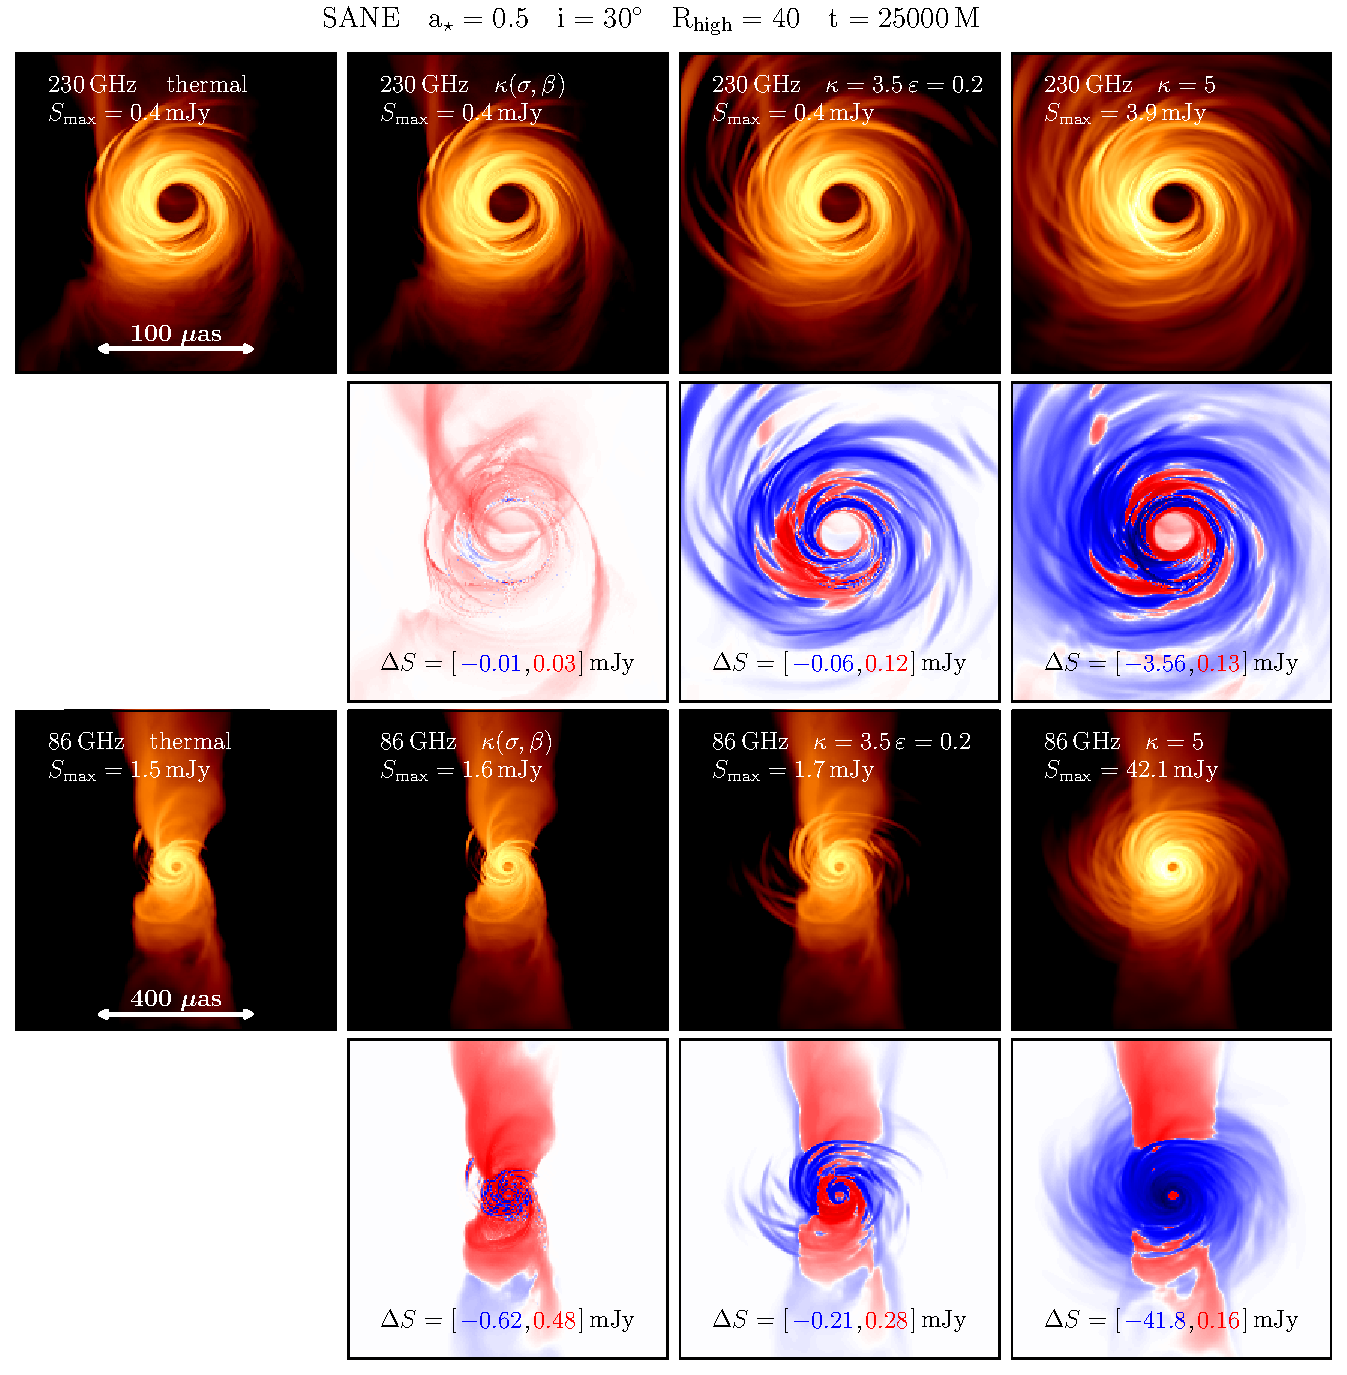
\includegraphics[width=\textwidth]{./figures/SANE_eDFs_diff.pdf}
  \caption{Influence of the eDF on the image structure for a SANE model with spin $a_{\star}=0.5$ seen under a viewing angle of 30$^\circ$ using $R_{\rm high}=40$ at t=25000\,M. In the first and third row the panels show the image structure from left to right a thermal, variable kappa $\kappa(\sigma,\beta)$, $\kappa=3.5$ (fixed) with efficiency $\varepsilon=0.2$ and $\kappa=5$ (fixed) everywhere eDF at 230GHz and at 86GHz. Notice the increased field of view for the 86\,GHz images. The second and fourth row show the difference between thermal image and the different non-thermal eDFs}
  \label{fig:SANE_edfs}
\end{figure*}

%\begin{figure}[t!]
%  \centering
%  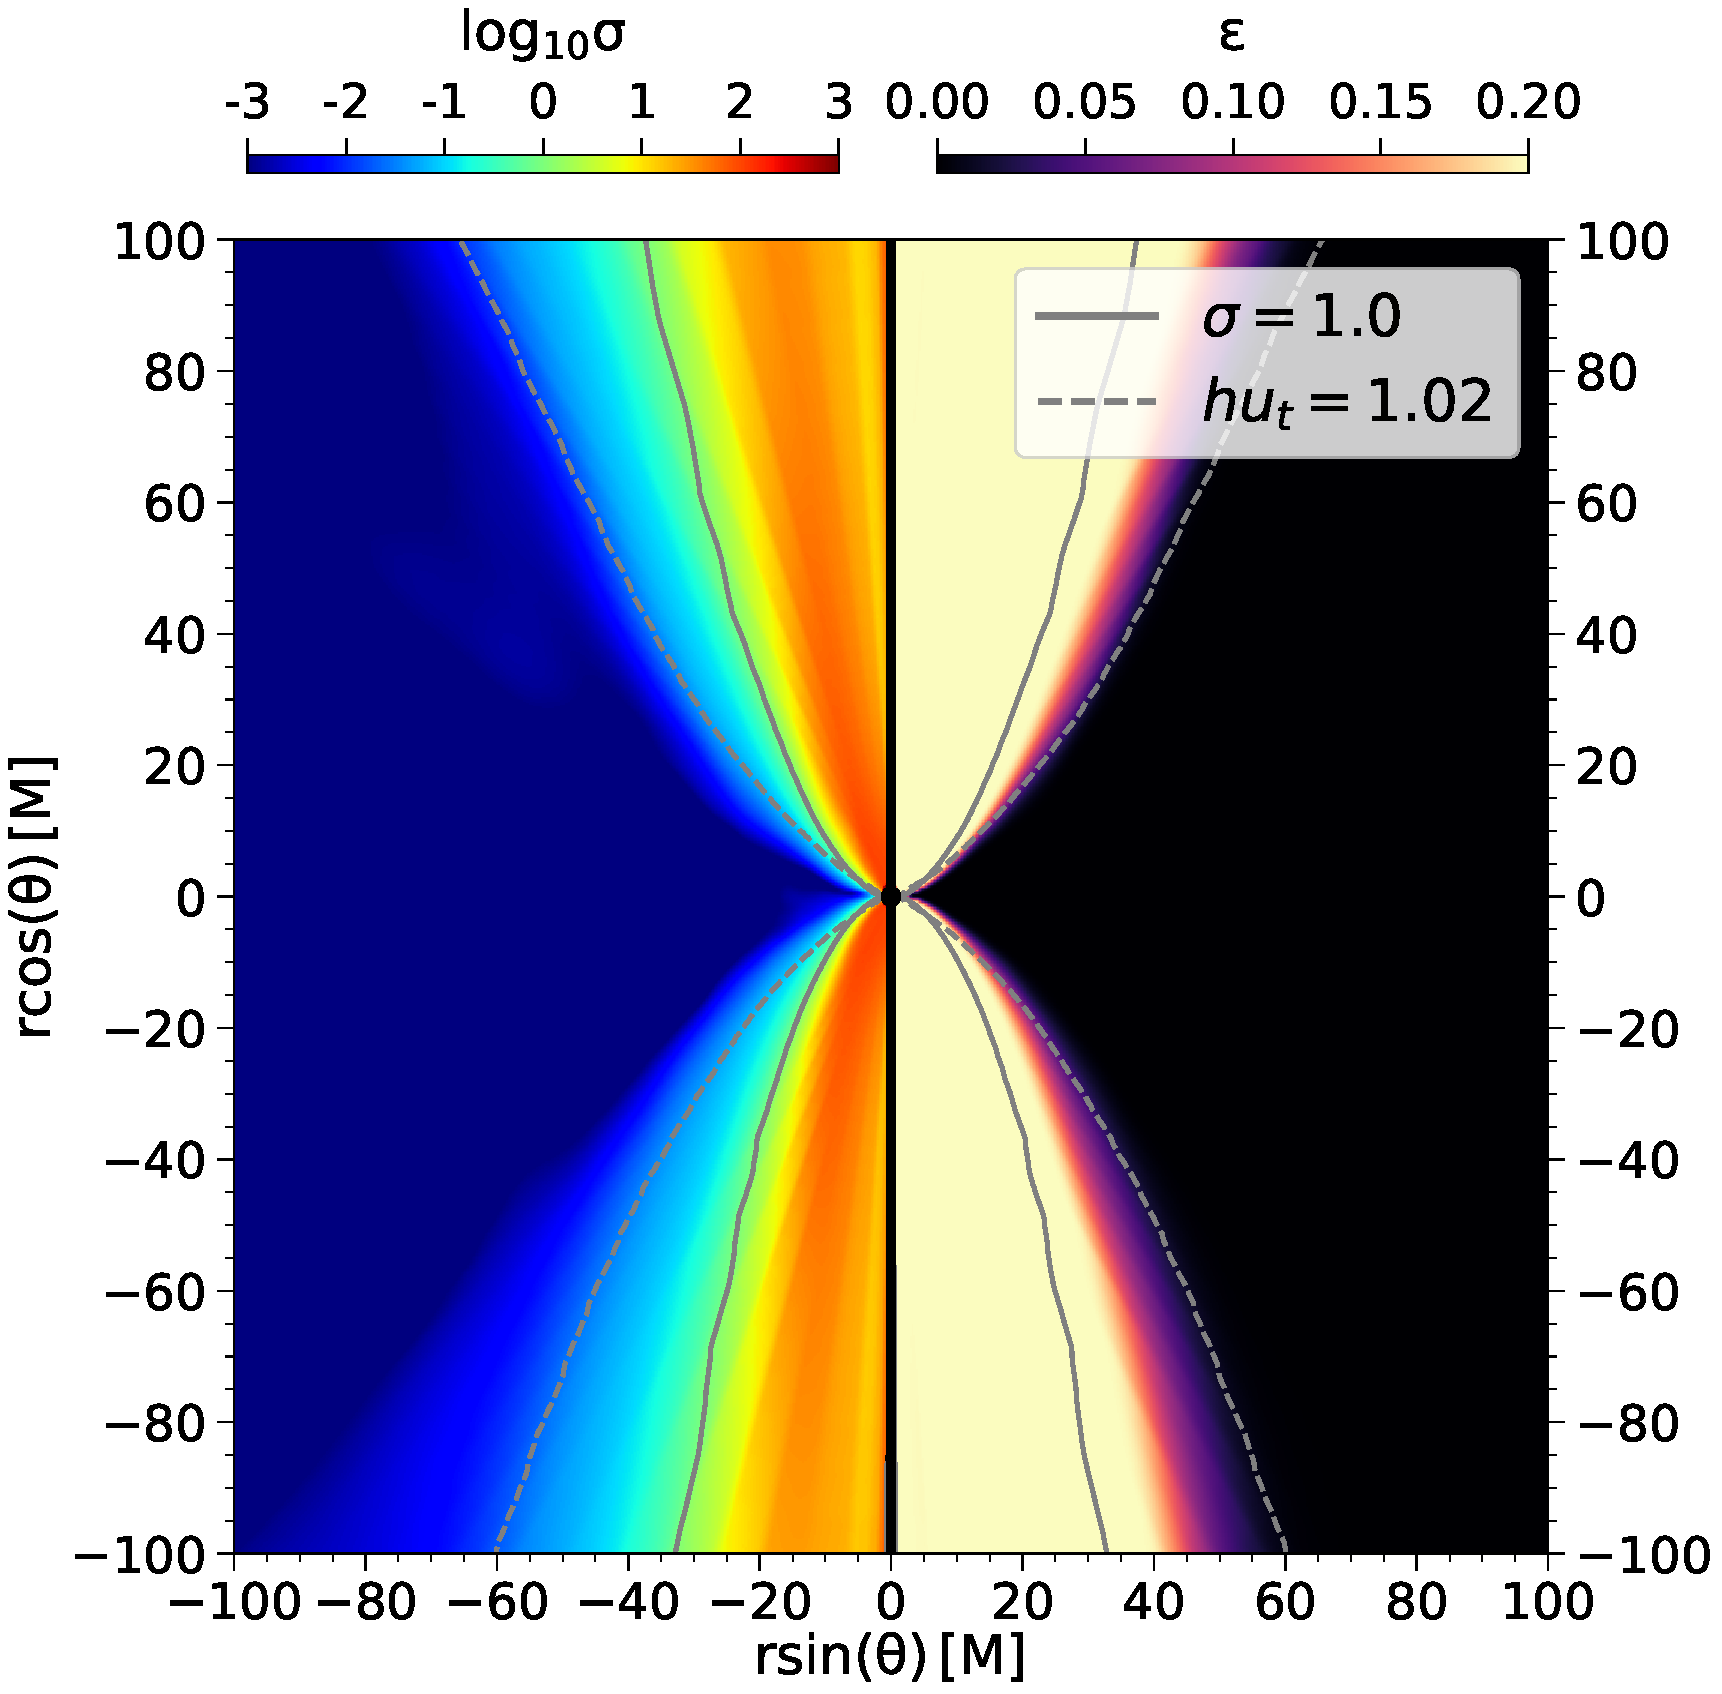
\includegraphics[width=\columnwidth]{./figures/GRMHDphiavera0.94sigmaeta.pdf}
%  \caption{Time and azimuthal averaged distribution of the magnetization, $\sigma$ (left half) and the efficiency, $\epsilon(\varepsilon,\beta,\sigma)$ using $\varepsilon=0.2 $ for a \bhac MAD GRMHD simulation with $\abh=0.94$. The solid gray line corresponds to $\sigma=1$ and the dashed line indicates out-flowing plasma via the Bernoulli parameter ($-h u_{t}>1.02$).
%  \ckc{Should we move this figure to the model section, as a way to demonstrate how the GRMHD and eDF look like?}}
%  \label{fig:varepsilon}
%\end{figure}

%In the following we will elaborate on the impact of adding non-thermal particles via the $\kappa$ electron distribution with fixed $\kappa$ value ($\kappa=3.5$) and three different base efficiencies $\varepsilon=$0.05, 0.1 and 0.2 on the observational constraints listed in Section~\ref{subsec:thermal}.
\subsubsubsection{230\GHz size and Lightcurve Variability}
\label{varkappa230}
For this model, the addition of non-thermal particles does not substantially affect the flux or size of the image at 230\GHz. For MAD models, 230\GHz emission is mostly produced in the disk region (see \citetalias{M87PaperV} and Fig.~8 in \citealt{Wong_2022} for a 3-D rendering).  Thus, the images are unaffected by the non-thermal particles, which are located in the jet. For SANE models, increasing $\Rh$ pushes the emission towards the jet sheath which increases the source size for high spins and large $\Rh$. However, the effect of non-thermal particles on the image is minor, because most of the emission is still produced by thermal electrons with temperature set by the $\Rh$ prescription (compare first and third panel in top row of Fig.~\ref{fig:SANE_edfs}). The passing fraction for the 230\GHz image size is 98\% independent of the efficiency, $\varepsilon$, which is consistent with 98\% of the thermal models fulfilling the image size constraint. We find that the 47\% of the models are in agreement with the 230\GHz variability constraint. This passing fraction is larger than for the thermal models (27\%). This discrepancy is most likely an effect of the shorter time window (5\,kM) considered for the non-thermal models in contrast to 15\,kM for the thermal ones. 

\subsubsubsection{Null location and Visibility Amplitude Morphology}
The null location and VA morphology constraint are obtained from the 230\GHz images. Since 230\GHz images of the $\kappa=3.5$ models with variable efficiency are similar to the thermal models (see previous paragraph) the fraction of passing models for both the Null location and VA morphology are comparable. The three non-thermal models have an average passing fraction for the Null location of 80\% whereas 83\% of the thermal models pass. The VA morphology constrain is fulfilled by 72\% of the models for both thermal and non-thermal eDF.  

\subsubsubsection{M-ring fits}
Given that including non-thermal particles via the equations presented in Eq.~\ref{eq:efficiencybetasigma} does not change the image structure and variability properties of the 230\GHz images the M-ring fits provide the same passing fractions for the diameter (65\%), width (22\%) and asymmetry (95\%).

\subsubsubsection{86\GHz source size and flux}
The 86\GHz source is only slightly affected by the addition of non-thermal particles as compared to the thermal models. Only the SANE models with $R_{\rm high}\geq 40$ and $a^{\star}>0$ produce 86\GHz image sizes larger than the thermal SANE models. This effect can be seen in  first and third panel in the bottom row of Fig.~\ref{fig:SANE_edfs}. Notice the increased flux density in the jet sheath in the difference image (blue color). This trend increases with the efficiency and is reflected in the decreasing pass fraction: 56\% (for $\varepsilon=0.05,0.1$) and 55\% ($\varepsilon=0.2$) as compared to thermal models (59\%).  
A similar trend is found for the 86\GHz flux density. The non-thermal particles are mainly located in the jet and thus contribute to the 86\GHz flux. Again, jet dominated high spinning SANE models typically fail the 86\GHz flux constraint. With increasing efficiency i.e. adding more non-thermal particles the pass fraction decreases and we found the following fractions: 67\% ($\varepsilon=0.05$), 66\% ($\varepsilon=0.1$) and 63\% ($\varepsilon=0.2$). In contrast to a pass fraction of 68\% for the thermal models.
%..............................................................................
%\subsubsubsection{230\GHz VLBI pre-image size}

%The addition of non-thermal particles produces almost undetectable changes in the 230\GHz VLBI pre-image sizes for the MAD models and a minor effect for the SANE models.


%An increase in $\Rh$ suppresses the emission from particles in the disk (by decreasing the electron temperature) and thus enhances emission from jet.  Since most the non-thermal particles are located in the sheath of the jet their impact on the source size is largest if the bulk of the thermal emission is also produced there.

% CFG: this is confusing.  is it needed?
%In addition the thermal synchrotron emissivity decreases at high frequency as $j_{\nu}\propto \exp{\left(-(\nu/\nu_c)^{1/3} \right)}$ while for the $\kappa$ distribution as $j_{\nu}\propto \nu^{-(\kappa -2)/2}$. This implies that for the same electron temperature the non-thermal flux is compared to a thermal one higher and thus leads to a more extended jet structure for the models including non-thermal particles.

%In MADs, independent of the choice of $\Rh$, the emission is mostly produced in the disk region (see \citetalias{M87PaperV} and Fig.~8 in \citet{Wong_2022} for a 3-D rendering).  Increasing $\Rh$ will not push the emission region into the jet where the non-thermal particles are located and thus their contribution to the total emission structure is negligible.

%..............................................................................
%\subsubsubsection{86\GHz Flux and Source Size}

% cfg 12-dec: this has already been mentioned elsewhere
%The 86\GHz GMVA+ALMA observations
%probe a larger field of view than the 230\GHz EHT observations, so we increased the field of view for the 86\GHz to 800\,$\rm{\mu as}$ during the radiative transfer calculations. Again the non-thermal particles are mainly located in the jet sheath and thus the increased field of view ensures that no extended flux is missing during the comparison with the 86\GHz observations.

%The 86\GHz flux density for both SANE and MAD models is unaffected by the addition of non-thermal particles.  There is a small effect for SANE models with $\Rh>40$, but even for $\varepsilon = 0.2$ this does not change which models are rejected.  Similarly the 86\GHz major axis FWHM is unaffected by the addition of non-thermal particles.

%n case of the SANE models the edges of the 86\GHz flux distribution are slightly shifted in the case of $\Rh>40$. However, including non-thermal particles even with the highest base efficiency $\varepsilon=0.2$ does not change the scoring of a model, i.e., a thermal-only model which full-fills the 86\GHz constrain is still accepted if non-thermal particles are included.

%This behaviour can be explained by the fact that the bulk of the emission in both accretion models is generated in with a few gravitational radii. Since the non-thermal particles are mainly located in the jet sheath and thei ratio between non-thermal to thermal particles is at most 20\% the contribution of the non-thermal particles to the 86\GHz flux can be neglected.

%..............................................................................
%\subsubsubsection{86\GHz image size}

%The behaviour of the 86\GHz image size is very similar to the above described 230\GHz image size: There is no change in image size for the MAD models and only a minor increase in the SANE models for $\Rh>40$. The physical reasons for this behaviour follows the same arguments as in the 230\GHz VLBI pre-image size.

%..............................................................................
\subsubsubsection{$2.2\um$ Constraint}

The addition of non-thermal electrons increases the $2.2\um$ flux for all models. For SANE models, except $\Rh=1$, the addition of non-thermal particles leads to over-production of $2.2\um$ photons. For MAD models, all models over-produce at $2.2\um$ for $\varepsilon \ge 0.05$. As noted above, $2.2\um$ emission is produced from the tail of the eDF.  The thermal eDF tail decreases exponentially, while the $\kappa$ eDF tail decreases as a power law, so the increase in $2.2\um$ flux density is unsurprising.  This is a general feature of the non-thermal models: $2.2\um$ observations sharply limit the allowed population of non-thermal electrons.

% commented out 12-dec, cfg: we should show trends in some model and some test other than this one, since we can easily make the case that the NIR increases as $\varepsilon$ increases.
%\begin{figure*}
%  \centering
%  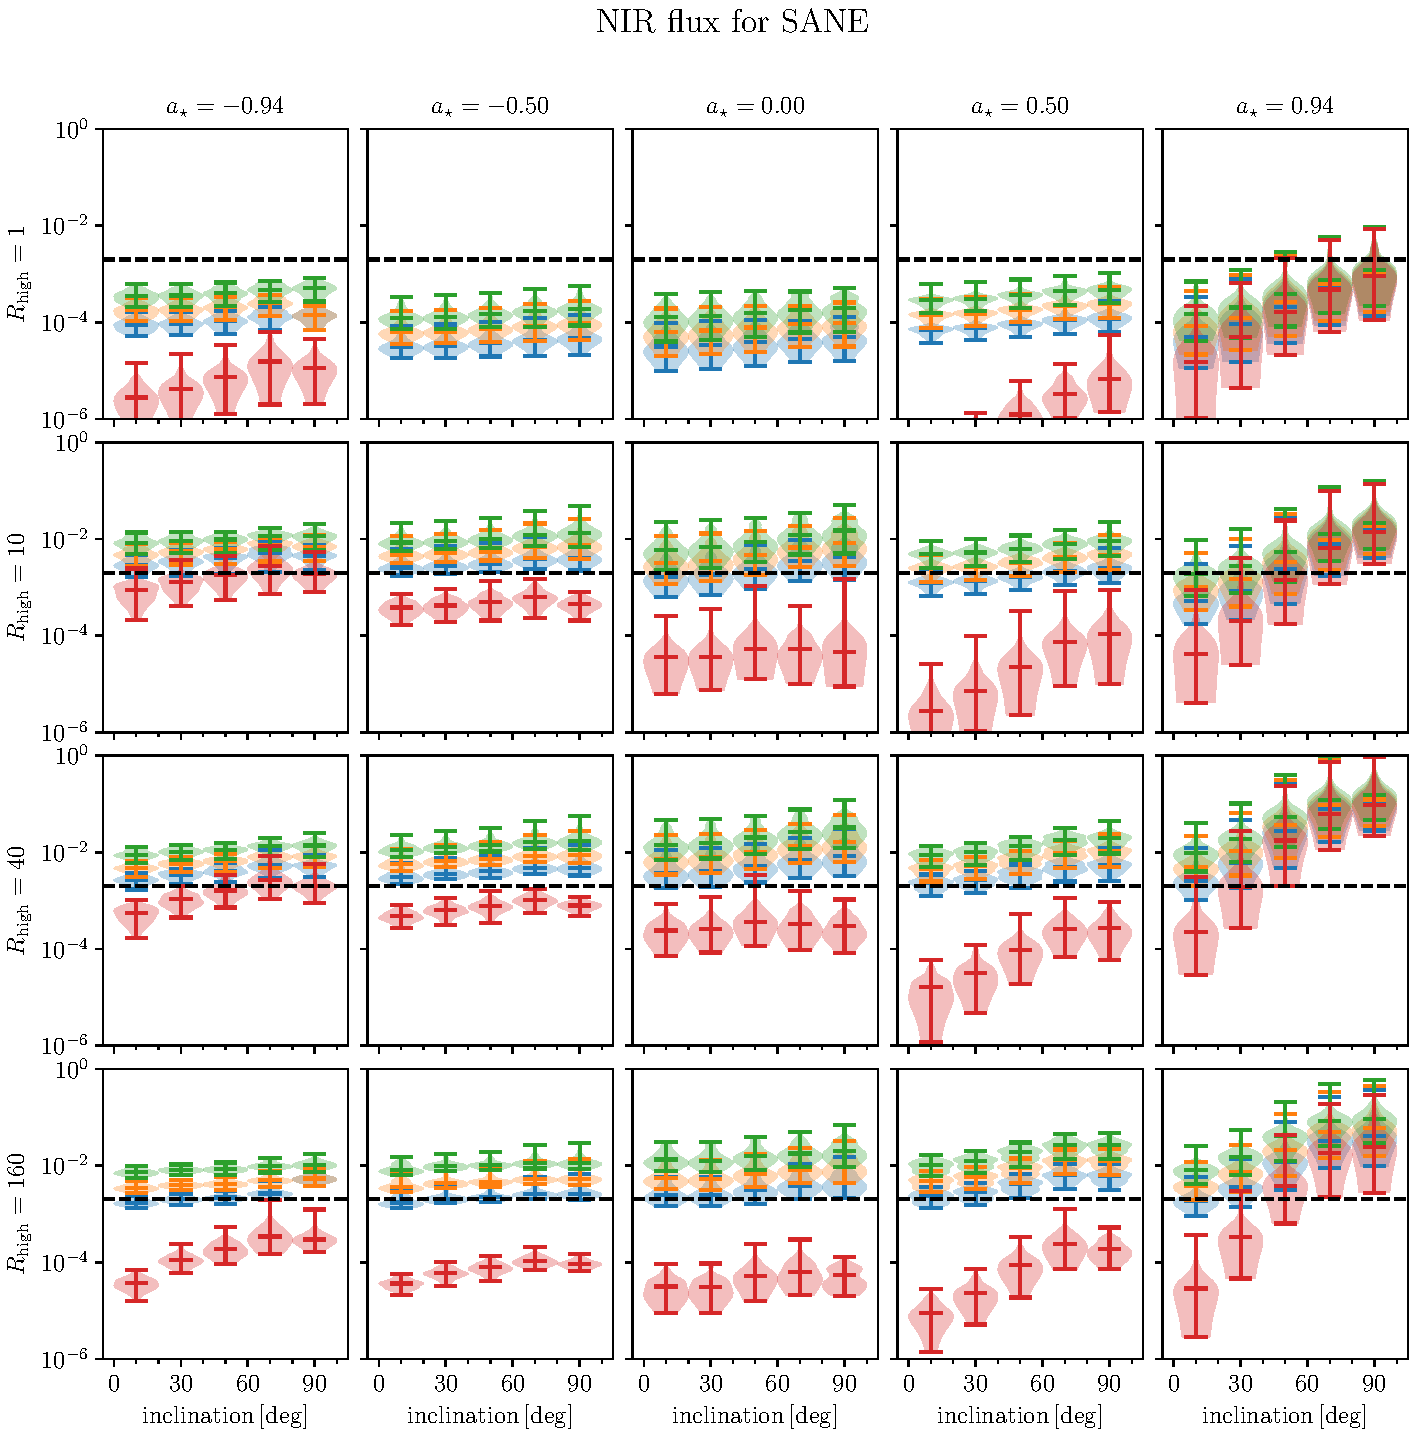
\includegraphics[width=0.8\textwidth]{./figures/SANE_NIR_standard.pdf}
%  \caption{Impact of non-thermal electrons on NIR flux constraint for the \bhac/\bhoss variable nonthermal efficiency model. NIR flux distributions are shown for SANE accretion models with thermal and non-thermal eDF with fixed $\kappa=3.4$ and $\epsilon\left(\sigma,\beta,\varepsilon\right)$ defined by Equation~\ref{eq:efficiencybetasigma}. The red violin plots correspond to a thermal eDF, blue, orange and green indicate $\kappa$ eDF with $\varepsilon=$0.05,0.1 and 0.2. The horizontal dashed line is the observational constraint.}
%  \label{fig:NIR_kappaepsilon}
%\end{figure*}



%..............................................................................
%\subsubsubsection{Lightcurve Variability}

%We compute $mi{3}$ for a window of $\num{5000}\tg$.  Notice that this is shorter than the standard models, which as three $\num{5000}\tg$ windows, so the results are less constraining.  The $\mi{3}$ test rejects about 1/2 of models for $\varepsilon = 0.05$, $0.1$, and $0.2$.  We conclude that $\varepsilon$ has no effect on the $\mi{3}$ test.

%For the comparison with the ALMA lightcurves we compute the modulation index for a 3\,hour time window and across the entire simulated time window of 28\,hours (5000\,GM/c$^3$). Similar to the 86\GHz flux the 230\GHz flux is mainly produced within a few gravitational radii and thus not affected by the addition of non-thermal particles using Eq. \ref{eq:kappaeff}. As in the previous constraints, the MAD accretion models are insensitive to the addition of non-thermal particles whereas the SANE models show some increased modulation index for $\Rh>40$. However, the distributions for thermal and non-thermal eDF are still largely overlapping.

%..............................................................................
%\subsubsubsection{\Mring Constraint}

%The \mring fitting is applied to the 230\GHz images. As mentioned earlier the flux and size of the 230\GHz images are not affected by the inclusion of non-thermal particles with fixed $\kappa$ and variable efficiency. Thus, we do not expect any changes in the distribution of the \mring parameters.  Applying \mring fitting to non-thermal models and a detailed comparison with the thermal results confirmed our initial assumption.

%\cmf{based on the results of Kotaro, who run the \mring on non-thermal models}

%------------------------------------------------------------------------------
\subsubsection{Variable \texorpdfstring{$\kappa$}{kappa} Model}

%\cfg{could we avod the equation and simply provide a reference and enough detail that someone could reproduce it?}\aco{What about inline equations?}

The high-energy variability observed in many astrophysical sources including the galactic centre could be explained by magnetic reconnection. During the reconfiguration of the magnetic field topology energy stored in the magnetic field is diffused into the plasma leading to the heating and acceleration of particles and finally resulting in the development of a non-thermal tails in the electron distribution functions. Particle in Cell (PIC) simulations have found that the slope of the non-thermal tail depends on the magnetisation of the plasma and its plasma-beta \citep[see, e.g.,][]{2018ApJ...862...80B}. Given that the magnetisation and plasma-beta vary within our GRMHD models we include as an alternative procedure for assigning a non-thermal eDF a $\kappa$ model \eqref{eq:nonthermaleDF} with variable $\kappa$ value and $w$ according to \cite{2018ApJ...862...80B}.
%, who model the effects of particle acceleration in magnetic reconnection.
In particular, we set
\begin{align}
  \kappa &= 2.8 +0.7\sigma^{-1/2} + 3.7\sigma^{-0.19}\tanh{(23.4\sigma^{0.26}\beta)}, \label{eq:kappa}\\
  w      &= \frac{ \kappa -3 }{\kappa} \Theta_e.
\end{align}

We use the emissivity and absorptivity, computed numerically for the interval $3 < \kappa \le 8$, from  \cite{2016ApJ...822...34P}. For $\kappa > 8$ we substitute a thermal eDF.  As in the fiducial models we turn off emission at $\sigma > 1$.
{The variable $\kappa$ models are computed from \hamr and \bhac GRMHD models where the time windows $30-35$\,kM (\hamr) and $25-30$\,kM (\bhac) are used. For the radiative transfer \ipole is applied to the \hamr models and the GRRT code \bhoss is employed for the \bhac models. For both models an image is created every 10\,M and we iterate the mass unit to obtain an average flux of 2.4\,Jy at 230\,GHz. In order to obtain the X-ray luminosity of the models, the monte carlo radiative transfer code \grmonty is connected to the \hamr models.}\\
%\cmf{The following text is for the \bhac models}
The required mass accretion rate to obtain 2.4\,Jy increases on average by 4\% as compared to the thermal. The larger mass accretion rate increases the number density of electrons, $n_e$, and thus the variable kappa models are slightly optically thicker than the thermal models.
\subsubsubsection{230\GHz size and Lightcurve Variability} The $kappa$ eDF is mainly applied in the jet sheath while the disk region is mostly populated by thermal particles. Therefore, the 230\GHz source size of the variable $\kappa$ models is similar to the thermal ones and no difference in the pass fraction is found. 98\% of the both models are in agreement with the 230\GHz size estimate (see first and second panel in the top row of Fig.~\ref{fig:SANE_edfs}). With a passing fraction of 30\% a slightly larger number of $\kappa$ models show the same lightcurve variability as the observations (27\% for thermal models).

\subsubsubsection{Null location and Visibility Amplitude Morphology} For the null location of the variable $\kappa$ models we find no difference to their thermal counterparts and for both $\sim$80\% pass this constraint. However, there is a clear discrepancy between the variable $\kappa$ and thermal models regarding the VA morphology. Only 60\% of the $\kappa$ models pass the VA morphology constraint, in contrast to 72\% of the thermal models.  

\subsubsubsection{M-ring fits}
Similar to the Null location and 230\GHz size constraint the thermal and variable $\kappa$ models agree in the passing fraction for the m-ring diameter (66\%), m-ring width (22\%) and asymmetry (95\%). 

\subsubsubsection{86\GHz source size and flux}
The number of models which are in agreement with 86\GHz source size are comparable for both thermal (59\%) and variable $\kappa$ models (55\%). Given that most of the variable $\kappa$ models are optically thicker than their thermal counter parts the 86\GHz flux is on average lower which increases the passing fraction from 68\% (thermal eDF) to 75\% (variable $kappa$ eDF).

\subsubsubsection{2.2\um Constraint}
Including non-thermal particles via the $\kappa$ eDF increases the 2.2\um flux as compared to the thermal eDF. The power law slope of the $kappa$ eDF depends on the magnetisation and plasma beta of the plasma (see Eq.~\ref{eq:kappa}). Since high magnetisation are typically found in MAD accretion models most of the MAD overproduce the 2.2\um flux. On the other hand in the low magnetised SANE models Eq.~\ref{eq:kappa} leads to large $\kappa$ values i.e., less high-energy electrons in the tail of the eDF. Therefore, the passing fraction for the SANE models is almost the same as for their thermal counter-parts. In total 35\% of the variable $\kappa$ models pass the 2.2\um constraint which should be compared to 55\% for models including only thermal particles.

\subsubsubsection{X-ray constraint}
As mentioned earlier, for the \hamr models we computed the x-ray luminosity. Including non-thermal particles via the variable $\kappa$ eDF reduces the passing fraction from 61\% (for thermal eDF) to 35\%. This behaviour is agreement with our expectations since the $\kappa$ eDF provides a larger reservoir of high energy electrons contributing to the up-scattering of photons.   
\subsubsubsection{Trends a across \bhac and \hamr models for variable $\kappa$ models}
For the variable $\kappa$ models two set of models from the \bhac and \hamr codes were used. Given the different adiabatic indices used (see Table \ref{tab:GRMHDmodels}) a direct comparison between the models is difficult. However, both models show similar trends for all constraints (see above paragraphs and Table~\ref{tab:passfraction}) except for the lightcurve variability and the VA morphology. For the \hamr models there is an increase of 21\% in the passing fraction for the lightcurve variability if non-thermal particles are included. Similar but not as pronounced for the variability constraint the fraction of passing models for the VA morphology increases from 39\% to 48\% if non-thermal particles are present.
%\aco{Add here details for ipole and igrmonty.}
%..............................................................................
%\subsubsubsection{Null Location} We found that $80\% ~(201/250)$  pass the expected null location ($2.5\lambda - 3.5G\lambda$). The differences to the thermal models can be described as follows: higher inclinations are rejected for $i \geq 70^{\circ}$ (MAD)  and $i \geq 50^{\circ}$ (SANE). Although, the total number of rejected models is similar to thermal models.

%..............................................................................
%\subsubsubsection{4 \texorpdfstring{$G\lambda$}{Gl} Visibility Amplitude Variability} In case of the variability at 4 $G\lambda$ 151/200 pass the constraint, same percent as for the thermal models, for instance $\sim 40 \%$ of the models are rejected, mostly negative $a_{\star} = -0.94$ SANE and MAD, also high temperatures, $R_{\rm high} = 160$, $a_{\star} \leq 0$ MAD accretion models, and  $i \geq 70^{\circ}$  for SANE prograde models.
%}

%\cfg{need very brief discussion here of the codes and run durations}

%\cfg{this section needs to incorporate both the \hamr and \bhac variable $\kappa$ models}

%\aco{
%The addition of nonthermal particles increases the X-ray emission from the majority of MAD models, causing them to overshoot the constraints. It does not change the general behavior of weak magnetic field SANE models.
%..............................................................................
%\subsubsubsection{86\GHz Major Axis}
%\michi{This description doesn't seem to correspond to what I see for either the BHAC or the HAMR variable $\kappa$ vs. thermal comparison}
%We found that the 86\GHz image size is similar to the thermal and variable efficiency models, differing only for non-spinning black holes, where we have low magnetization, weak jet. As a consequence our prescription makes $\kappa$ large and the radiative properties of the plasma similar to those of a thermal eDF. eDF with variable $\kappa$ power-law reduces to thermal distribution and the size of the image is a bit smaller than in thermal case. For $a_{\star}=0$ almost all SANE models pass the size constraint, $R_{\rm high}=1$ we have a bit larger image. For MAD $R_{\rm high}=40$ and $a_{\star}=0.94$, and cases for $R_{\rm high}=160$ and $a_{\star}=0.50$ we have a bit smaller size image than thermal case passing the constraint.

%..............................................................................
%\subsubsubsection{86\GHz flux}

%\michi{This description doesn't seem to correspond to what I see for either the BHAC or the HAMR variable $\kappa$ vs. thermal comparison}
%The total flux on overall non-thermal models increases in comparison to thermal models, however, the general results for MAD models do not change. For SANE models with R$_{\rm high}=1$ slightly increases, all of them fail in contrast with thermal models. While for $R_{\rm high}=10,40,80$ and $R_{\rm high}=160$ the flux decreases under the lower bound $1.8 \rm {Jy}$.

%..............................................................................
%\subsubsubsection{NIR constraints}

%\michi{This description doesn't seem to correspond to what I see for either the BHAC or the HAMR variable $\kappa$ vs. thermal comparison}
%The contribution of non-thermal electrons at the NIR emission produce larger flux in all models, independent on black hole spin, inclination angle or electron temperature. For MAD accretion models with $a_{\star}=0$ and $R_{\rm high}=1$ only small inclination $i=10\degree$ pass the constraint. While models with $R_{\rm high}=10,40$ overshooting GRAVITY mean flux, again for thermal case these models satisfy the constraint. On the other hand, since for non-spinning black hole the jet is no well developed and the magnetization is low, for only  $R_{\rm high}=80$, $a_{\star}=0.5$ and $30^{\circ} \leq i$ survive, similar behavior for $R_{\rm high}=160$ and spins $|a_{\star}|=0.5$.
%Larger emission than thermal models excludes SANE models for $R_{\rm high}=10$ and $\abh < 0$ as well as  $R_{\rm high}=40,~80$ and $\abh \leq 0.0$. While even larger NIR flux the models for $R_{\rm high}=160$ are still under the threshold.

%..............................................................................
%\subsubsubsection{ALMA lightcurves}

%We compute the the modulation index  of the lightcurves of variable $\kappa$ models by discretizing the entire window of GRMHD simulations, $\rm 5000\,\tg$ ($\rm 28\,hours$) every $\rm 3\,hour$ (see Table \ref{tab:GRMHDmodels}). Similar to variable efficiency models, the non-thermal particles with variable $\kappa$ has not big impact on the flux at 230\GHz. The behavior of modulation index and total flux for MAD accretion models are same as thermal, and variable efficiency eDFs. We found sightly high modulation index for $R_{\rm high}=1$ and $30^{\circ} \leq i$ for SANE accretion models, the models for $R_{\rm high}=80$ has same trend as $R_{\rm high}=40$.

%------------------------------------------------------------------------------
\begin{deluxetable*}{l|ccccccc}\label{tab:passfraction}
\tablecaption{Exploratory Model Pass Fractions}
\tablehead{
\colhead{constraint/model}		 &		
\colhead{}		 &		
\colhead{\bhac}		 &		
\colhead{}
\colhead{}
\colhead{\hamr }
\colhead{}
\colhead{}
}
\startdata
	& Thermal & $\kappa(\sigma,\beta)$& $\kappa=3.5\,\varepsilon=0.05,0.1,0.2$& $\kappa=5$ & Thermal & $\kappa(\sigma,\beta)$ & $p = 4$ \\
\hline
230\,GHz size				&	0.98   &	 		0.99			& 		0.98,0.98,0.98		 	& 		0.92		  &	1.0		& 		0.99		 	& 		0.94	\\
VA Morphology		     	&	0.27   &	 		0.80			&  		0.81,0.81,0.78			& 		0.59		  &	0.07	& 		0.88			&  		--		\\
M-ring diameter				&	0.72   &	 		0.69			&  		0.66,0.66,0.67			& 		0.71		  &	0.39	& 		0.67			&  		0.89	\\
M-ring width		    	&	0.83   &	 		0.21			&  		0.24,0.23,0.23			& 		0.03		  &	0.80	& 		0.40			&  		0.13	\\
M-ring asym.		   		&	0.65   &	 		0.97			&  		0.95,0.95,0.94			& 		0.73		  &	0.61	& 		0.97			&  		0.98	\\
86\,GHz flux		    	&	0.21   &	 		0.75			&  		0.67,0.66,0.63			& 		0.12		  &	0.32	& 		0.65			&  		0.72	\\
86\,GHz size		   		&	0.95   &	 		0.57			&  		0.56,0.56,0.55			& 		0.38		  &	0.99	& 		0.45			&  		0.47	\\
2.2$\mu$m flux				&	0.59   &	 		0.35			&  		0.14,0.12,0.12			& 		0.14		  &	0.46	& 		0.25			&  		0.41	\\
X-ray flux					&	0.68   &	 		--				& 		--						& 		--		  	  &	0.62	&  		0.35			& 		--		\\
lc varability				&	0.55   &	 		0.30			&  		0.47,0.47,0.46			& 		0.29		  &	0.80	& 		0.28			&  		0.41	\\
4G$\lambda$ variability		&	0.70   &	 		0.60			&  		0.74,0.73,0.71			& 		0.55		  &	0.35	& 		0.46			&  		0.63	\\
EHT Constraints             & 		   &  		   ,   ,   			& 		   		  				& 		   			  &  		&						&				\\
non EHT Constraints         & 		   &  		   ,   ,   			& 		   		  				& 		   			  &  		&						&				\\
Variability Constraints     & 		   &  		   ,   ,   			& 		   		  				& 		   			  &  		&						&		   	    \\
\enddata
\tablecomments{Pass fractions for \bhac and \hamr models for varios eDFs}
\end{deluxetable*}



\subsubsection{Summary of Constraints on Non-Thermal Models}
In Table \ref{tab:passfraction} we list the pass fractions for \bhac and \hamr models using different eDFs.
Most non-thermal eDF models considered here produce little change compared to the thermal models for most constraints. The 86\GHz size and flux, which are the most important non-EHT constraints, are only marginally affected by the addition of nonthermal electrons. This behaviour is obtained especially for eDFs which mainly add non-thermal particles in jet while the disk is populated by thermal ones. In our case this setup is given for variable $\kappa$ and $\kappa=3.5$ with variable efficiency and is consistent between \bhac and \hamr models (see Table~\ref{tab:passfraction}).

If non-thermal particles are included also in the disk, either via a power-law with slope p=4 stitched to a thermal distribution or via a $\kappa=5$ distribution there are some variations in pass fractions as compared to the above-mentioned eDFs.
\newline For the power-law models the addition of non-thermal electrons increase the 86\GHz size by 50\%. However the pass fractions with respect to the thermal model is not changed. In contrast to the $\kappa=5$ models where pass fraction decreased by 20\% as compared to the thermal models.
\newline For both models, $p=4$ and $\kappa=5$ fewer models pass the 230\GHz m-ring width. We find a consistent decrease by $\sim20\%$ for both models. Interestingly the other m-ring constraints i.e., the diameter and asymmetry are not affected by the addition of non-thermal particles. This can be explained by the finer and brighter ring feature found in $p=4$ and $\kappa=5$ models connected to their smaller optical depth compared to their thermal counter-parts (see Table~\ref{tab:passfraction}). 
\newline In general the fraction of models passing the $\mi{3}$ increase with the addition of non-thermal particles independent on the prescriptions of the eDF %\cmf{for the \hamr models there is a large increase from 7\% to 41\% which I think will survive even if we would run all models longer. The change for the \bhac models is smaller and could be removed if the models are run for longer. How to include this?}
\newline The main characteristic of the non-thermal models is the increase of 2.2\um and X-ray flux densities. However, in a large fraction of models this leads to overproduction of 2.2\um or X-ray flux and reduces the pass fractions.\\

\begin{deluxetable*}{l|ccccc}\label{tab:fail_none}
\tablecaption{Exploratory models that pass all constraints}
\tablehead{
\colhead{Code/Setup} &
\colhead{MAD/SANE} &
\colhead{spin} &
\colhead{inc} &
\colhead{$\Rh$} &
\colhead{Constraint(s) failed at $15,000\tg$}
}
\startdata
\bhac $\kappa(\sigma, \beta)$	&	MAD		&	0.5		&	10		&	80 		& 	Mring width, \mi{3}		\\ 
\bhac $\kappa(\sigma, \beta)$	&	MAD		&	0.5		&	10		&	160		&	Mring width, \mi{3}		\\ 
\bhac $\kappa(\sigma, \beta)$	&	MAD		&	0.5		&	30		&	160		&	\mi{3}					\\ 
\hline
\bhac $\epsilon = 0.05$			&	SANE	&	0.94	&	10		&	10 		& 	\mi{3}					\\	
\hline
\hamr $p = 4$	  				&	SANE	&	0.94	&	50		&	40 		& 	2.2\,$\mu$m flux		\\	
\hamr $p = 4$	  				&	MAD		&	0.5		&	50		&	1 		&  	Mring diameter, \mi{3}
\enddata
\tablecomments{Exploratory models which pass all constraints when computed to $5,000\tg$. When extended to $15,000\tg$, each model fails one or more constraints. }

\end{deluxetable*}



If all constraints are considered six non-thermal models pass all constraints (see Table~\ref{tab:fail_none}). These models are: one \hamr MAD $p=4$ model with $a^\star=0.5$ seen under an inclination of 50$^\circ$ and  $R_{\rm high}=1$ and a high spinning SANE model with $a^\star=0.94$ at an inclination of 50$^\circ$ with $R_{\rm high}=40$. From the \bhac variable $\kappa$ three models are in agreement with all constraints namely: spin $a^\star=0.5$ at inclination 10$^\circ$ at $R_{\rm high}=$80 and 160 and a model with the same spin seen under a slightly larger angle of $30^\circ$ with $R_{\rm high}=160$. The last of the six survivors is a \bhac SANE model with variable efficiency of  $\varepsilon=0.05$ with an inclination of 10$^\circ$ and a $R_{\rm high}=10$. All of these models share a common low inclination angle $\leq 60^\circ$ and large positive spin. The MAD models agree with the cluster of thermal models found for both \bhac and \kharma models (see Sect.~\ref{sec:summarythermal}).
%\cmf{there is one \bhac SANE $\varepsilon=0.05$ with spin $a^\star=0.94$, inclination 10$^\circ$, and $R_{\rm high}=10$ which only fails M3. However this one would fail most likely the polarisation constraint. How do include this here? }

\begin{deluxetable*}{l|ccccc}\label{tab:fail_one}
\tablecaption{Exploratory models that fail only one constraint}
\tablehead{
\colhead{Code/Setup} &
\colhead{MAD/SANE} &
\colhead{spin} &
\colhead{inc} &
\colhead{$\Rh$} &
\colhead{Constraint Failed}
}
\startdata
\bhac $\kappa(\sigma, \beta)$	&	SANE	&	0		&	70		&	1		&	86\,GHz flux		\\	  
\bhac $\kappa(\sigma, \beta)$	&	MAD		&	0.5		&	10		&	40		&	2.2\,$\mu$m flux	\\	  
\bhac $\kappa(\sigma, \beta)$	&	SANE	&	0.5		&	10		&	40		&	\mi{3}   			\\	  
\bhac $\kappa(\sigma, \beta)$	&	SANE	&	0.5		&	10		&	80		&	\mi{3}   			\\	  
\bhac $\kappa(\sigma, \beta)$	&	SANE	&	0.5		&	10		&	160		&	\mi{3}   			\\	  
\bhac $\kappa(\sigma, \beta)$	&	SANE	&	0.5		&	30		&	40		&	\mi{3}   			\\	  
\bhac $\kappa(\sigma, \beta)$	&	SANE	&	0.5		&	30		&	80		&	\mi{3}   			\\	  
\bhac $\kappa(\sigma, \beta)$	&	SANE	&	0.5		&	30		&	160		&	\mi{3}   			\\	  
\bhac $\kappa(\sigma, \beta)$	&	MAD		&	0.5		&	30		&	80		&	\mi{3}   			\\	  
\bhac $\kappa(\sigma, \beta)$	&	MAD		&	0.5		&	50		&	160		&	\mi{3}   			\\	  
\bhac $\kappa(\sigma, \beta)$	&	MAD		&	0.94	&	10		&	160		&	\mi{3}   			\\	  
\bhac $\kappa(\sigma, \beta)$	&	MAD		&	0.5		&	30		&	160		&	\mi{3}				\\	  
%\bhac $\kappa(\sigma, \beta)$	&	MAD		&	0.5		&	10		&	80		&	??					\\	%This fail two constraints, but only in the extended 15kM runs  
%\bhac $\kappa(\sigma, \beta)$	&	MAD		&	0.5		&	10		&	160		&	??					\\	%This fail two constraints, but only in the extended 15kM runs   
\hline
\bhac $\epsilon = 0.05$			&	SANE	&	0.94	&	10		&	10		&	\mi{3}   			\\	
\bhac $\epsilon = 0.05$			&	SANE	&	0.94	&	30		&	10		&	86\,GHz flux   		\\	
\bhac $\epsilon = 0.05$			&	MAD		&	0.5		&	30		&	160		&	2.2\,$\mu$m flux   	\\	
\bhac $\epsilon = 0.05$			&	MAD		&	0.5		&	50		&	160		&	2.2\,$\mu$m flux   	\\	
\bhac $\epsilon = 0.05$			&	MAD		&	0.94	&	10		&	40		&	2.2\,$\mu$m flux   	\\	
\hline
\bhac $\epsilon = 0.10$			&	SANE	&	0.94	&	10		&	10		&	2.2\,$\mu$m flux   	\\	
\bhac $\epsilon = 0.10$			&	MAD		&	0.5		&	30		&	160		&	2.2\,$\mu$m flux   	\\	
\bhac $\epsilon = 0.10$			&	MAD		&	0.5		&	50		&	160		&	2.2\,$\mu$m flux   	\\	
\bhac $\epsilon = 0.10$			&	MAD		&	0.94	&	10		&	40		&	2.2\,$\mu$m flux   	\\	
\hline
\bhac $\epsilon = 0.20$			&	SANE	&	0.94	&	10		&	10		&	2.2\,$\mu$m flux   	\\	
\bhac $\epsilon = 0.20$			&	MAD		&	0.94	&	10		&	40		&	2.2\,$\mu$m flux   	\\	
\bhac $\epsilon = 0.20$			&	MAD		&	0.94	&	10		&	160		&	2.2\,$\mu$m flux   	\\	
\hline
\bhac $\kappa = 5$				&	MAD		&	0.94	&	50		&	1		&	2.2\,$\mu$m flux   	\\	
\hline
\hamr 30$^\circ$ tilt  			&	INSANE	&	0.94	&	10		&	160		&	86\,GHz size		\\	
\enddata
\tablecomments{Models which pass all of the constraints except for one. Since no model passes all constraints, these represent the parameters that are closest to being consistent with observations.}

\end{deluxetable*}


%The exception is for the powerlaw models, where the addition of nonthermal electrons increases the 86GHz size by 50\%. \cmf{howerver, the pass fraction is not changed}

%The 230\GHz \mring fits are hardly affected at all by the addition of nonthermal electrons using the prescriptions considered here, and $\mi{3}$ is also not substantially affected by the addition of nonthermal electrons.



%Since the nonthermal models analyzed here do not consider the heating efficiency due to the magnetic reconnection, $\varepsilon \neq 0$, those effects can be explained by asymptotic behaviour of the nonthermal emissivity, $ j_{\nu}\propto\exp\left(-\Theta_e^{-2/3}\nu^{1/3}\right)+\nu^{-(\kappa-2)/2} \left[(\kappa -3)\Theta_{\rm e} + \varepsilon(\kappa -3) \sigma\right]^{\kappa-2}$. The second term dominates at NIR and X-rays, while at mm and radio frequencies the first term dominates. However, as soon as heating efficiency in the third term becomes nonzero, the nonthermal contribution generates a larger emission region, expanding the image size at 86\GHz,  and increasing the total intensity \citep{2021NatAs.tmp..218C,2021arXiv211102518F}. Furthermore, both the NIR and the X-ray average flux increases as efficiency increases.
%on the other hand, the SED is not sensitive to the black hole spin but image size increase for prograde models, we have consistency overall our models (\bhac / \hamr).

%The effect of adding non-thermal electrons in a $\kappa$ eDF with  $\kappa=3.4$ and variable efficiency via Eq.~\ref{eq:efficiencybetasigma} can be summarized as follows:
%\begin{itemize}
 %   \item The 86\GHz and 230\GHz constraints are hardly affected by the addition of non-thermal particles.
%    \item Even the lowest base efficiency considered, $\varepsilon=0.05$, leads to an over-production of NIR flux. \cmf{indication that we need very localised regions of non-thermal particle productions and no "global" approach?}
%\end{itemize}

%Adding nonthermal electrons in the form of a power-law results in a definite increase in 230 and 86\GHz image sizes. Very few models survive all constraints: one SANE accretion model with black hole spin $a_{\star}=15/16$, $\rm R_{high}=40$ at an inclination of $50^{\circ}$ passes EHT, non-EHT and variability tests. A couple of MAD spin $a_{\star}=0.5$ models also pass EHT and non-EHT constraints.


%The effect of adding nonthermal electrons in a variable $\kappa$ eDF can be summarized as follows: Only $1\%$ of models pass all constrains, MAD accretion model, black hole spin $a_{\star}=0.5$, $\rm R_{high}=160\ (i=10^{\circ},~30^{\circ})$ and $\rm R_{high}=80\ (i=10^{\circ})$.%, see model C in Figure \ref{fig:bestbet_imgs}.

%The effect of adding nonthermal electrons in a constant-$\kappa$ model can be summarized as follows:


%Most of our nonthermal models assign a width to the nonthermal component that depends on the an electron `temperature assigned through the $\Rh$ scheme, so they are not fully independent of $\Rh$.

The nonthermal models are run for only $5000\tg$, so most  constraints can not be applied as precisely.  For example, the model distribution of $\mi{3}$ contains only $9$ points and is correspondingly more uncertain than for the thermal models.  It is therefore difficult to detect subtle changes in models.
%}

%==============================================================================
\subsection{Tilted Models}

The aligned models considered up to now are a special case: in general one would expect that the spin angular momentum of the black hole and the orbital angular momentum of the accretion flow would be misaligned. Here we consider misaligned flows around an $a_*=15/16$ black hole from \citet{Liska2018} and \citet{Chatterjee2020}.

All aligned models considered so far produce either a SANE or MAD accretion flow.  The tilted disk model initial conditions, however, produce a strongly magnetized near-MAD outcome with dimensionless magnetic fluxes between 25-50, a state known as IN-SANE.  We consider three GRMHD simulations with tilt $0^{\circ}$, $30^{\circ}$ and $60^{\circ}$.

The tilted models exhibit a warped disk due to the Lense-Thirring torques imposed by the black hole.  The time-averaged disk and jet are therefore non-axisymmetric.
%Notice that the jets are always approximately perpendicular to the outer disk in these models.
Since the inner and the outer disk have different orientations, it is necessary to specify the coordinate axis of the observer.  We consider three  observer inclinations with respect to the {\em outer} disk at a single azimuth of $0\degree$ \citep[for more details, see][]{Chatterjee2020}.\footnote{A full parameter survey would run over azimuth angle as well.}  
%A full listing of the pass/fail results are given in Appendix~\ref{app:tables}, Table~\ref{tab:ThamrPF}.

The 230\GHz pre-image size of edge-on large $\Rh$ images increases slightly for the tilt-$60\degree$ compared to the aligned case. This occurs because the inner jet is warped and creates an extended image. This effect is also seen in the 86\GHz image size. On the other hand, the 86\GHz flux varies little with tilt despite the presence of a boosted jet component at large tilt angles.

% cfg 12-dec this is a testable proposition
%This suggests that, on average, most of the total flux at 230 and 86\GHz comes from a few gravitational radii from the black hole where the relativistic Doppler boost have comparable values between the in-going accretion flow and the out-flowing jet.

Variability increases with the tilt. In tilted disks, accretion occurs via thin plunging streams \citep[e.g.,][]{Fragile2007} where electrons in the shocked flow can be heated to relativistic temperatures \citep[e.g.,][]{Dexter2013, 2014ApJ...780...81G, White2019}, forming localized, fluctuating hotspots more easily than in aligned disks, thereby increasing flux variability \citep{Chatterjee2020, 2021arXiv210412896W}.

% cfg: added white & quat ref below.  already got white et al. 2019 above [if I have the correct one], and added generozov as 2014ApJ...780...81G
%\smr{Should we cite other works on tilted accretion flows (e.g., Generozov+ 2013, https://arxiv.org/abs/1311.5565, White et al 2019, https://arxiv.org/abs/1902.09662, White \& Quataert 2021, https://arxiv.org/abs/2104.12896)?}

%\cfg{Statement about which models pass and fail MI}
%\kc{
These models generally fare well with the $\mi{3}$ constraint with 20/27 models passing. A few models with $\rm R_{high}=160$ and one model with $\rm R_{high}=40$ fail.  This does not mean that tilted models are less variable, however, since the the constraints on \mi{3} are more than a factor of 2 weaker for the $3000\tg$ integrations considered than for the $15 \times 10^3\tg$ integrations used in our fiducial models.
%}

$2.2\um$ flux also increases with tilt.  The $2.2\um$ flux exceeds the 1.0 mJy limit for all 3 tilts, with a few exceptions, e.g., $R_{\rm high}=160$ models at $10^{\circ}$ inclination, which makes it difficult to favor the aligned case over the tilted one. Furthermore, the presence of misalignment destroys the axisymmetric nature of the accretion flow.  The current model set covers a small parameter space in inclination and $R_{\rm high}$.  A thorough exploration of the source azimuthal angle with respect to the observer is left to future studies.

To summarize: for the model set considered here tilt primarily affects variability and the $2.2\um$ flux density, tending to increase both and thus shifting acceptable aligned models into rejected models as tilt angle increases.  These trends are consistent with those observed by \cite{2021arXiv210412896W}.

%==============================================================================
\subsection{Stellar Wind Fed Models}

The accretion models of \cite{2020ApJ...896L...6R, 2020MNRAS.492.3272R, 2018MNRAS.478.3544R} track plasma from  magnetized stellar winds down to the event horizon and provide a self-consistent picture of the origin of both gas and magnetic fields in the accreting plasma in \sgra.  The resulting inflow does not fully circularize, so the models also provide a distinct alternative to the fiducial models, which {\em assume} that the torus initial conditions relax to an astrophysically accessible state for the inner accretion flow.  Recall that in the wind-fed models the density of the wind is fixed, so the 230\GHz flux density is matched to observations by varying $\Rh$ instead.  

We consider two versions of the model: one in which the stellar wind magnetization is low ($\beta = 10^6$) and a second in which the magnetization is high ($\beta = 10^2$). $\Rh$ is adjusted until each model has the observed time-averaged 230\GHz flux density, with $\Rh = 13$ ($\beta = 10^6$) and $\Rh = 28$ ($\beta = 10^2$).

Both wind-fed models fail the \mring width test, producing a width that is too small.  In addition both are too bright at 86\GHz, and fail the $\mi{3}$ test, although they are quieter than MAD models and close to the cutoff.   %All scoring results are given in Appendix~\ref{app:tables}, Table \ref{tab:resslerPF}.

Both non-EHT and EHT constraints have the power to test wind-fed models.  It is {\em not} possible to draw broad conclusions about the viability of the wind-fed models in general, however, since the two models tested here contain only a single spin ($a_\star=0$) and all use the $\Rh$ thermal eDF model.

